\lstinputlisting[language=bash,basicstyle=\small]{python_codes/fieldstone_78/keywords}

\begin{center}
Code at \url{https://github.com/cedrict/fieldstone/tree/master/python_codes/fieldstone_78}
\end{center}

\par\noindent\rule{\textwidth}{0.4pt}

%%%%%%%%%%%%%%%%%%%%%%%%%%%%%%%%%%%%%%%%%%%%%%%%%%%%%%%%%%%%%%%%%%%%%%%%%%%%%%%%%%%%%%%%%%%%%%%%%%%%


Although the $Q_1\times P_0$ is not LBB-stable (see Section~\ref{ss:LBBcond})
it has been proven that some spatial arrangements of this element can be, such as the
so-called Stenberg macro-element described in Section~\ref{ss:meshtopos}.
On the following a mesh is shown which consists of $16\times 16$ of such macro-elements:

\begin{center}
a)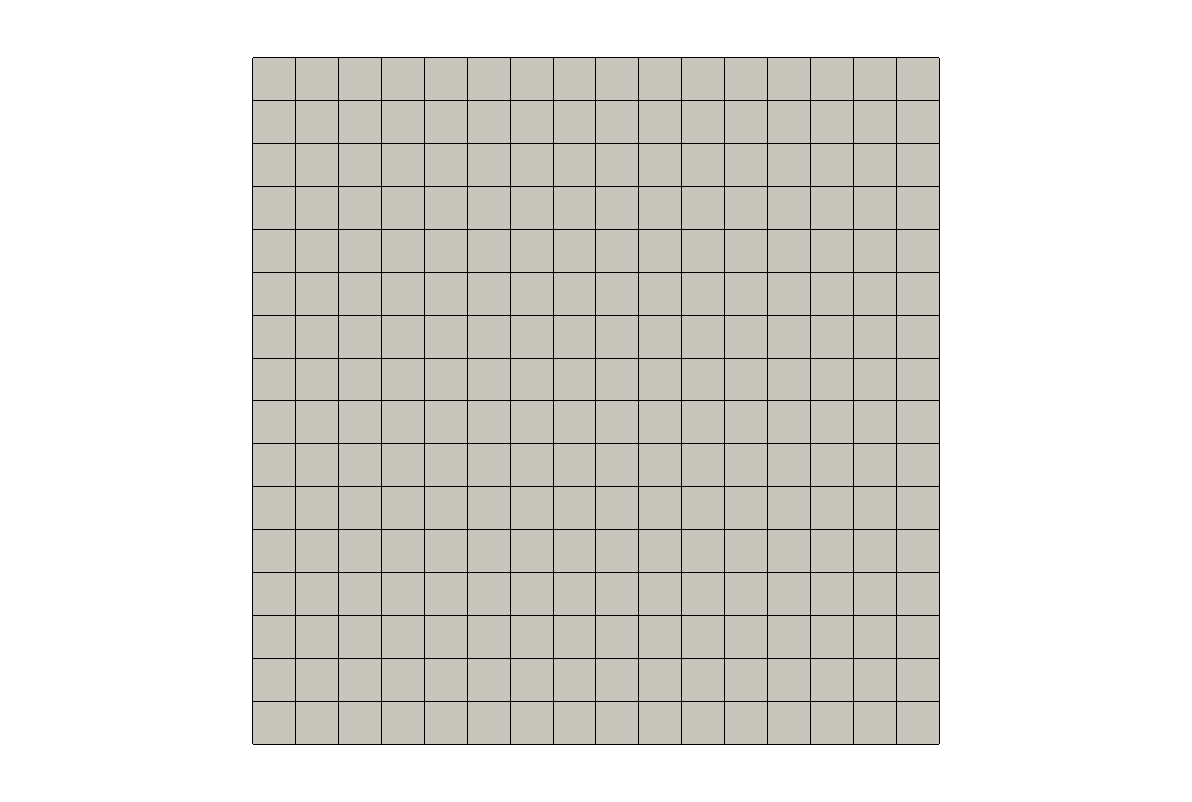
\includegraphics[width=4cm]{python_codes/fieldstone_78/results/mms_dh/16x16/grid0000}
b)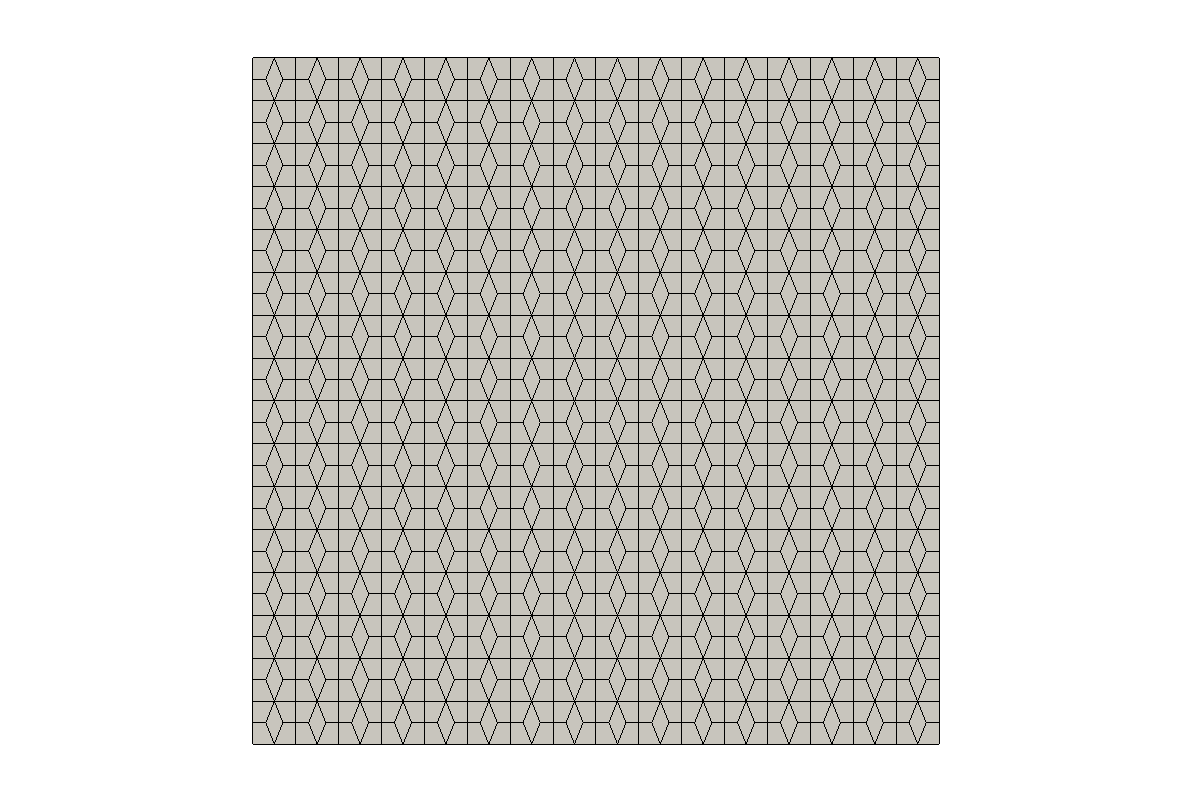
\includegraphics[width=4cm]{python_codes/fieldstone_78/results/mms_dh/16x16/grid0001}
c)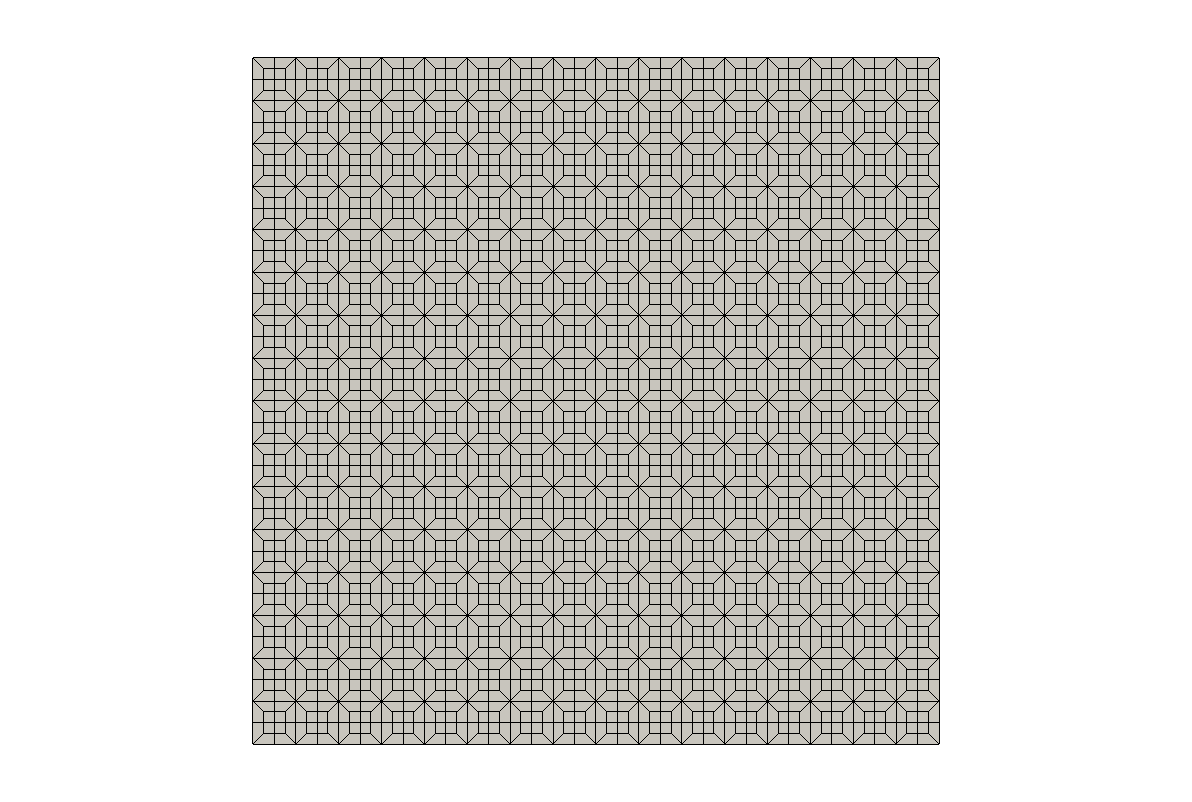
\includegraphics[width=4cm]{python_codes/fieldstone_78/results/mms_dh/16x16/grid0002}
d)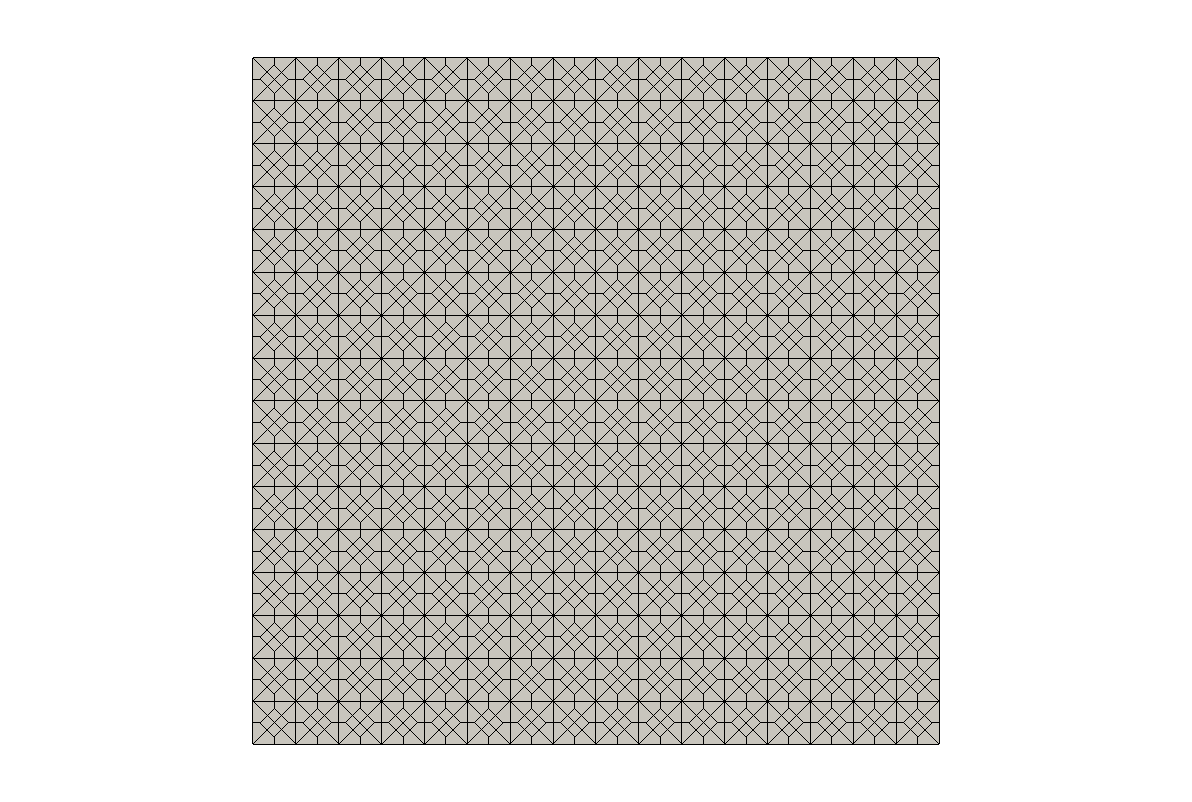
\includegraphics[width=4cm]{python_codes/fieldstone_78/results/mms_dh/16x16/grid0003}\\
e)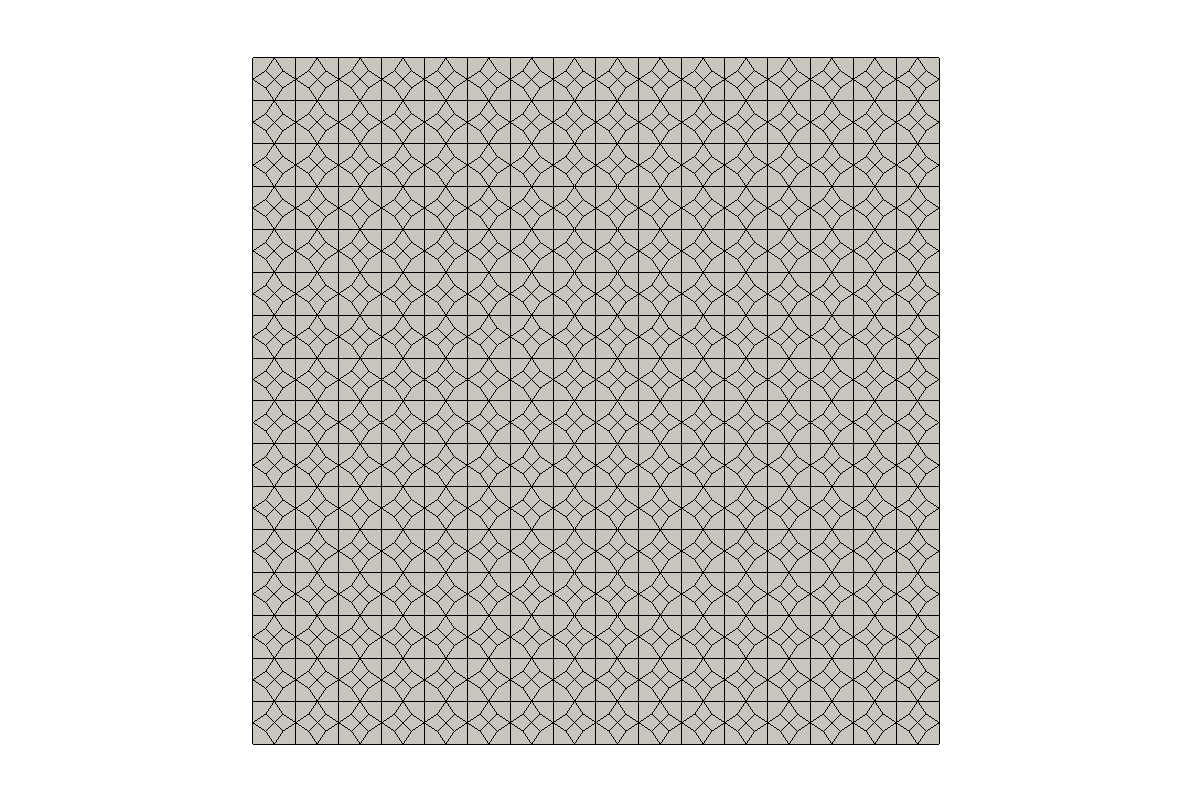
\includegraphics[width=4cm]{python_codes/fieldstone_78/results/mms_dh/16x16/grid0004}
f)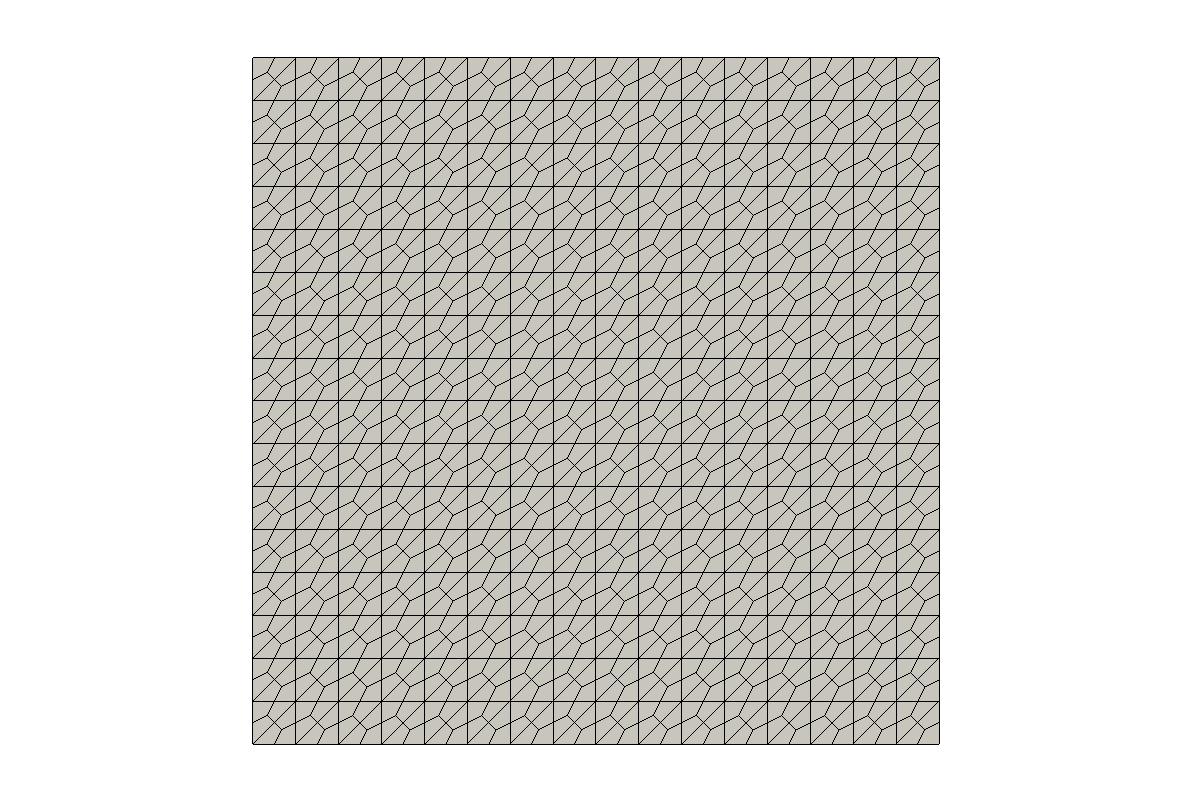
\includegraphics[width=4cm]{python_codes/fieldstone_78/results/mms_dh/16x16/grid0005}
g)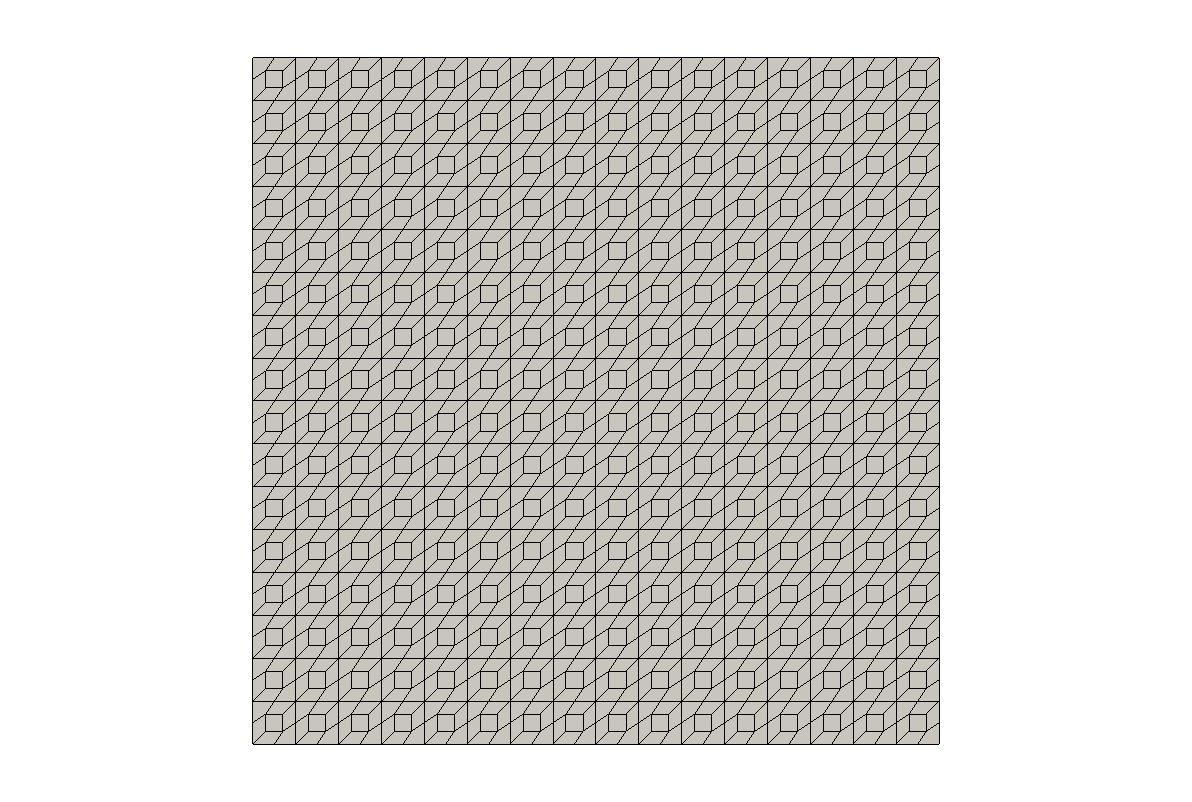
\includegraphics[width=4cm]{python_codes/fieldstone_78/results/mms_dh/16x16/grid0006}
h)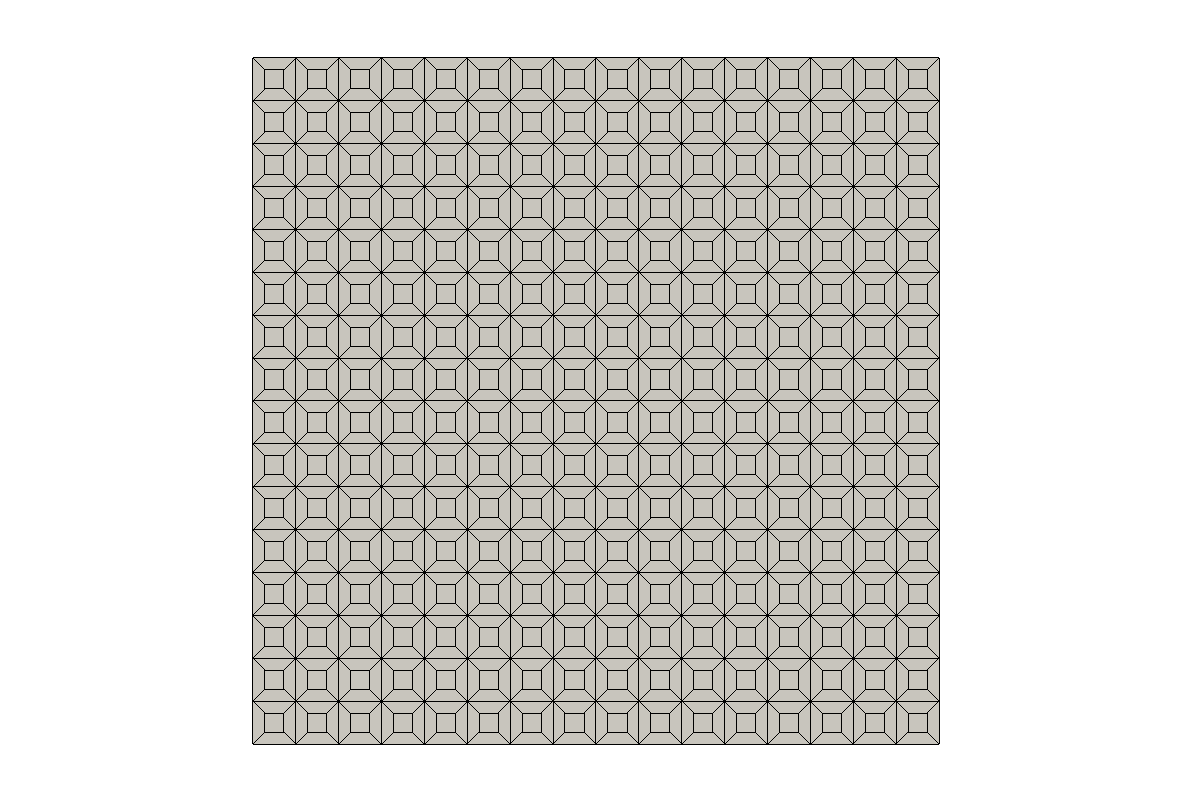
\includegraphics[width=4cm]{python_codes/fieldstone_78/results/mms_dh/16x16/grid0007}\\
{\captionfont  opla}
\end{center}

The meshes are created by importing the corresponding files:
\begin{lstlisting} 
import letallec
import stenberg
import qinzhang
import regular
\end{lstlisting} 
Inside each of these files a function called {\sl mesher} is defined: 
\begin{lstlisting} 
def mesher(Lx,Ly,nelx,nely,nel,NV,mV):
\end{lstlisting} 
The arguments are the domain size $L_x$ and $L_y$, the number of macroelements
in each direction $nelx$ and $nely$, the precomputed total number of $Q_1\times P_0$ 
elements $nel$ and nodes $NV$ and the number of nodes per element $m_\upnu$.  

Pressure normalisation is achieved by setting $p=0$ on the last element and then 
renormalising the pressure field so that $\int p dV=0$. In what follows $p$ is the 'raw' pressure
field while $q$ denotes its projection onto the nodes. 

%\begin{center}
%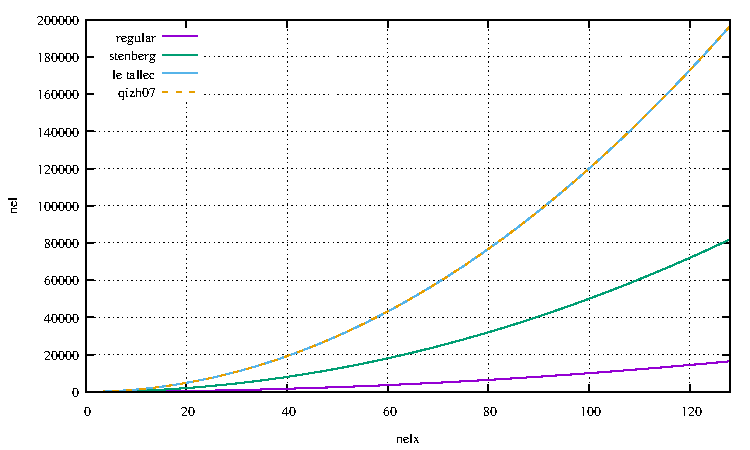
\includegraphics[width=7cm]{python_codes/fieldstone_78/images/nel}
%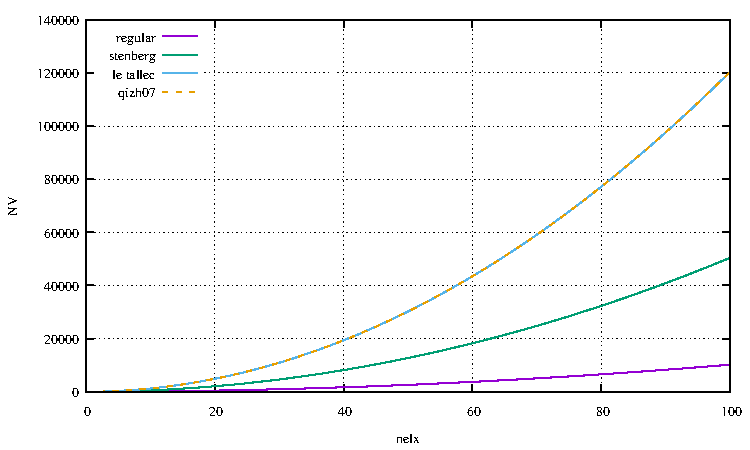
\includegraphics[width=7cm]{python_codes/fieldstone_78/images/NV}\\
%{\captionfont Total number of elements (left) and V nodes (right) as a function of the number
%of macro-elements in the $x$-direction (assuming $nelx=nely$.}
%\end{center}



%\begin{center}
%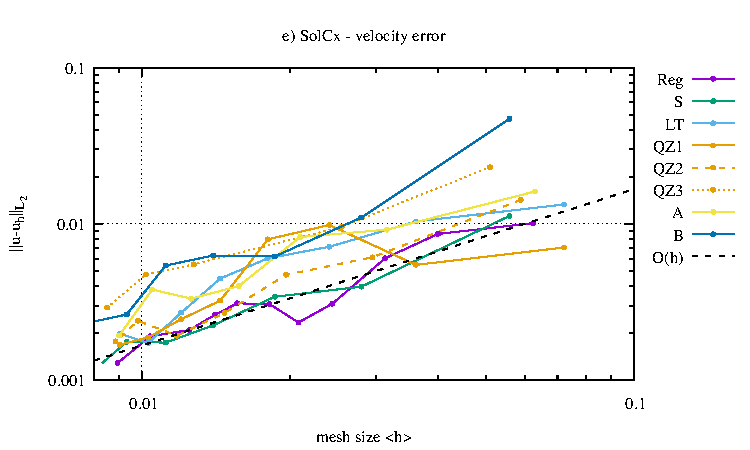
\includegraphics[width=4cm]{python_codes/fieldstone_78/results/mms/LR_eps/errors_V}
%{\captionfont Varying $\epsilon$ for LT macro-element at fixed 32x32 resolution. Vertical 
%line is value such that all elements have the same area.}
%\end{center}

{\color{red} note that the viscosity is evaluated in the middle of each element, not 
at the quadrature points. This can/will have an effect on non-isoviscous models.}


%........................
\paragraph{Results - mms}

We start with the Donea \& Huerta manufactured solution (see Section~\ref{mms1}) and 
proceed to compute the velocity and pressure error convergence as a function of the 
element size which is taken to be $h = \sqrt{L_xL_y/nel}$. We see that 
the errors converge as expected, quadratically for the velocity and linearly for the pressure.
Rather interestingly the projection of the pressure onto the nodes has a convergence rate 
higher than the raw elemental pressure. As predicted in Qin \& Zhang, the Stenberg macro-element 
yields the best results, followed by the Le Tallec and then the one they propose (this conclusion 
is logically supported by looking at root mean square velocity measurements). 
Finally, the presence of the checkerboard for the regular structure mesh case
makes it painfully clear that it is the worst mesh topology 
and the pressure error does not converge.  

\begin{center}
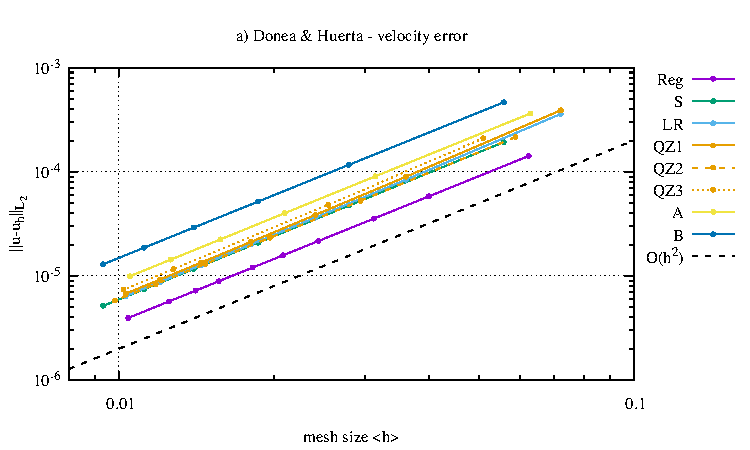
\includegraphics[width=5cm]{python_codes/fieldstone_78/results/mms_dh/errors_V.pdf}
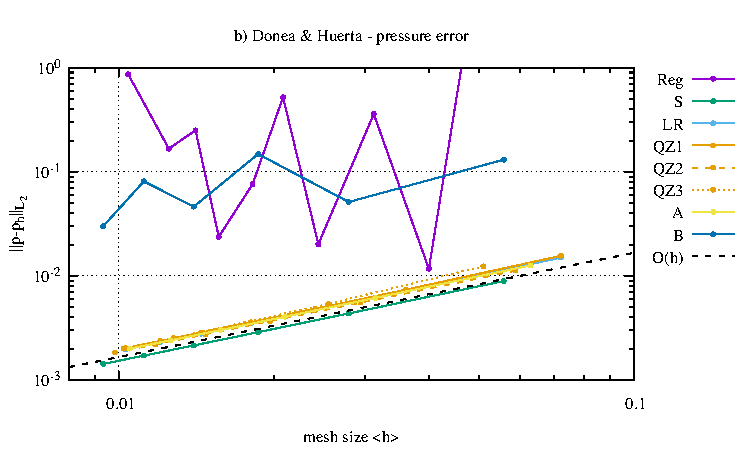
\includegraphics[width=5cm]{python_codes/fieldstone_78/results/mms_dh/errors_P.pdf}
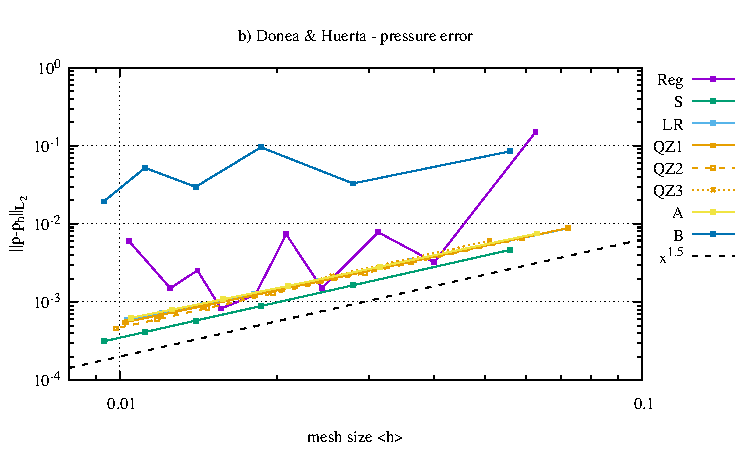
\includegraphics[width=5cm]{python_codes/fieldstone_78/results/mms_dh/errors_Q.pdf}\\
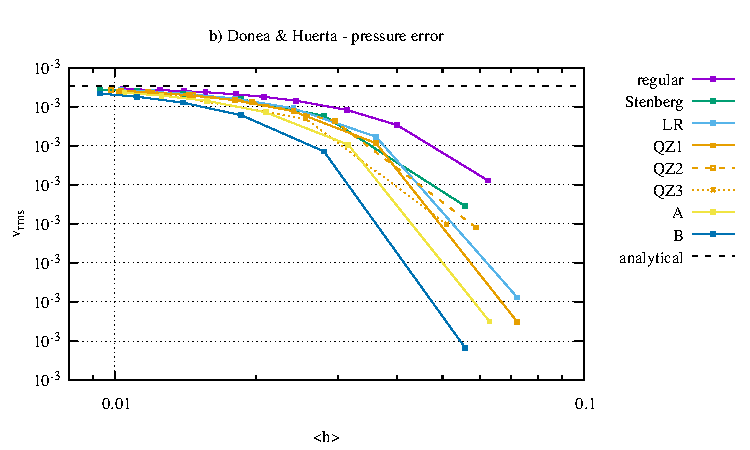
\includegraphics[width=8cm]{python_codes/fieldstone_78/results/mms_dh/vrms.pdf}
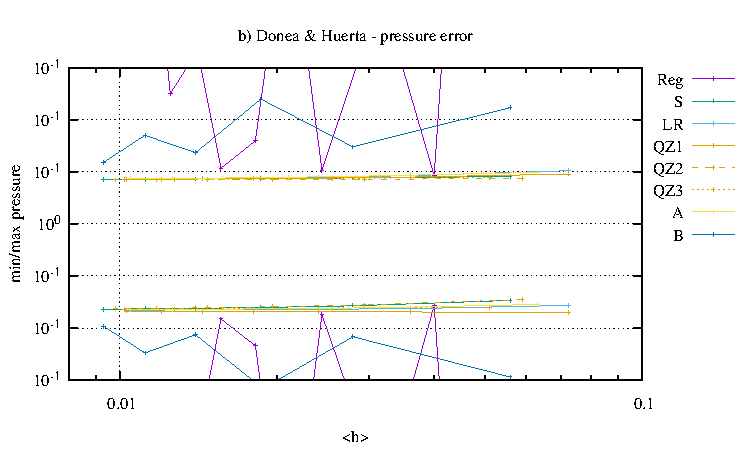
\includegraphics[width=8cm]{python_codes/fieldstone_78/results/mms_dh/pstats.pdf}
\end{center}

On the following figures the pressure is plotted against the analytical solution and 
we see that there is no checkerboarding occurring:
Rather interestingly the pressure error is the largest next to the boundaries:

\begin{center}
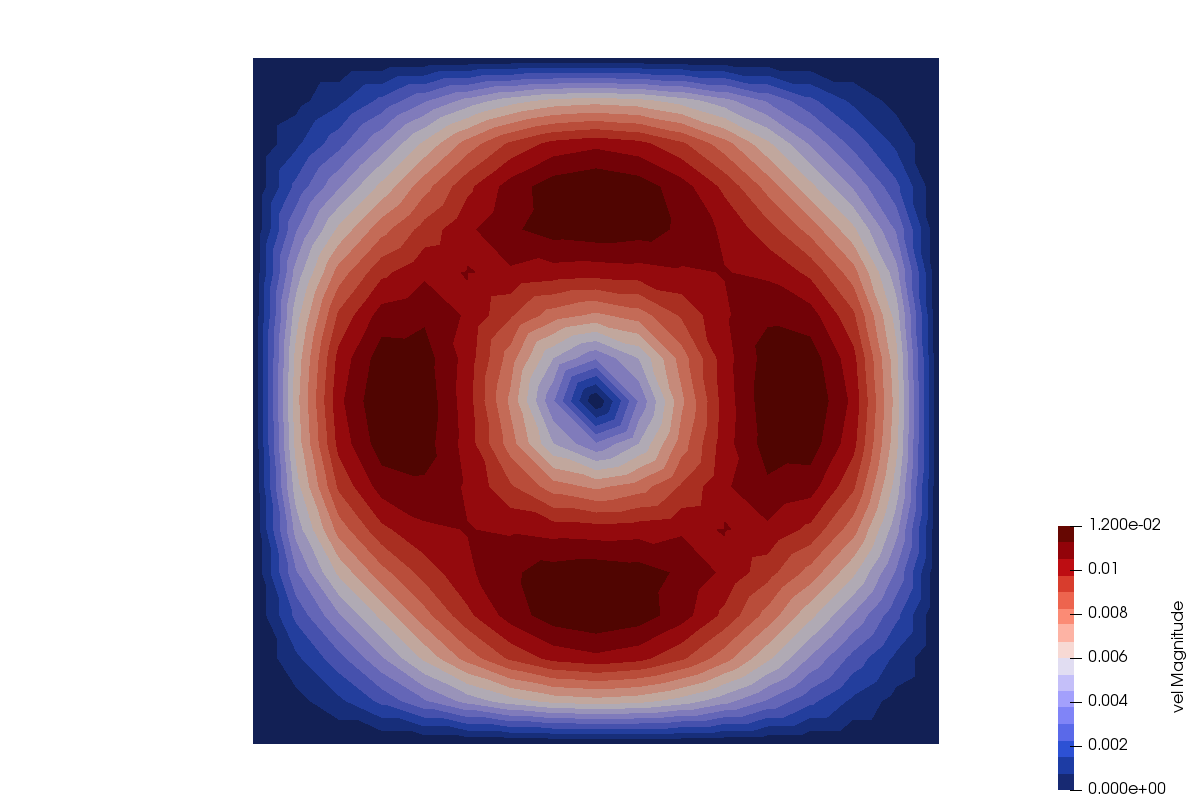
\includegraphics[width=4cm]{python_codes/fieldstone_78/results/mms_dh/16x16/vel0000}
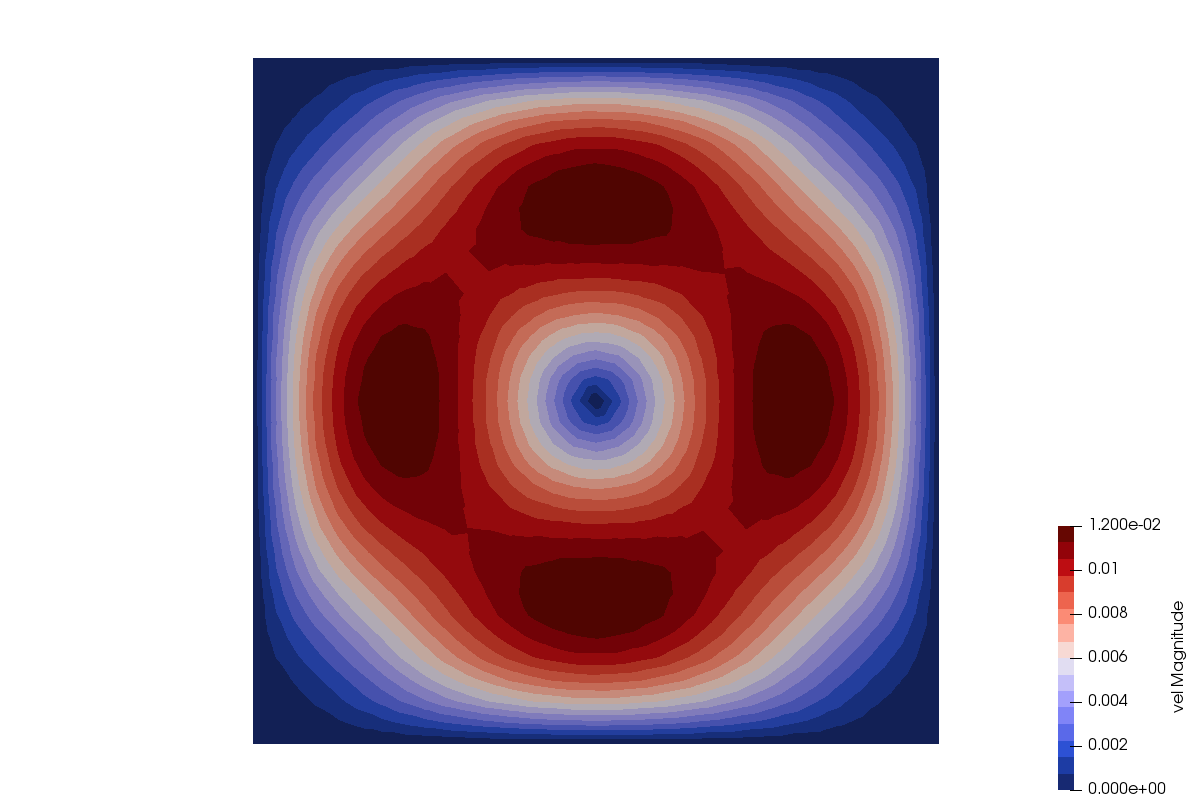
\includegraphics[width=4cm]{python_codes/fieldstone_78/results/mms_dh/16x16/vel0001}
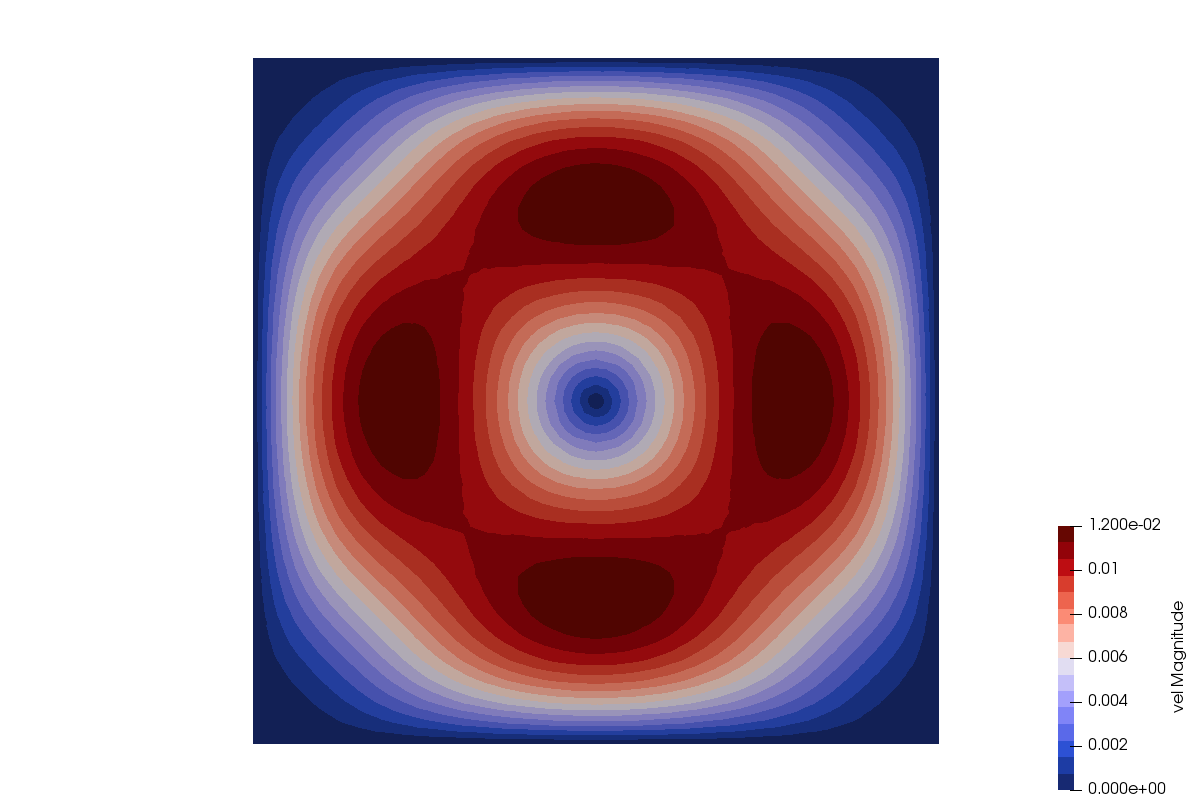
\includegraphics[width=4cm]{python_codes/fieldstone_78/results/mms_dh/16x16/vel0002}
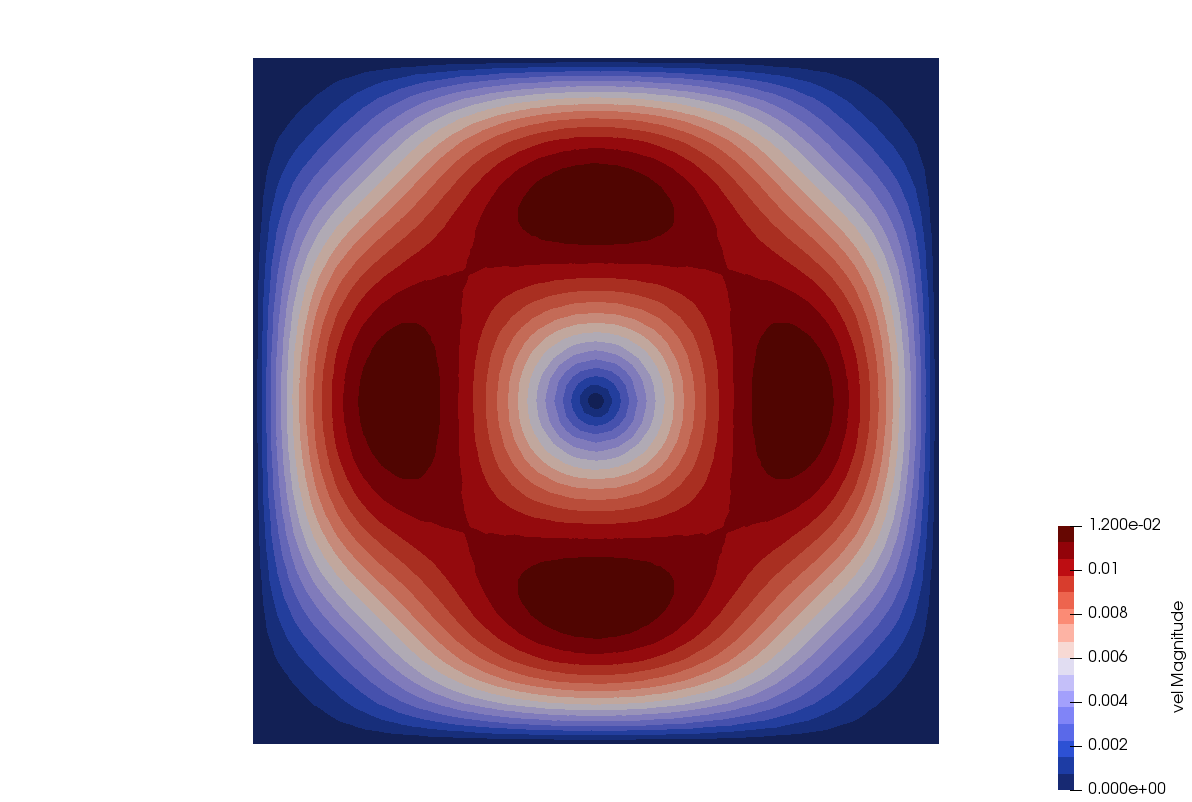
\includegraphics[width=4cm]{python_codes/fieldstone_78/results/mms_dh/16x16/vel0003}\\
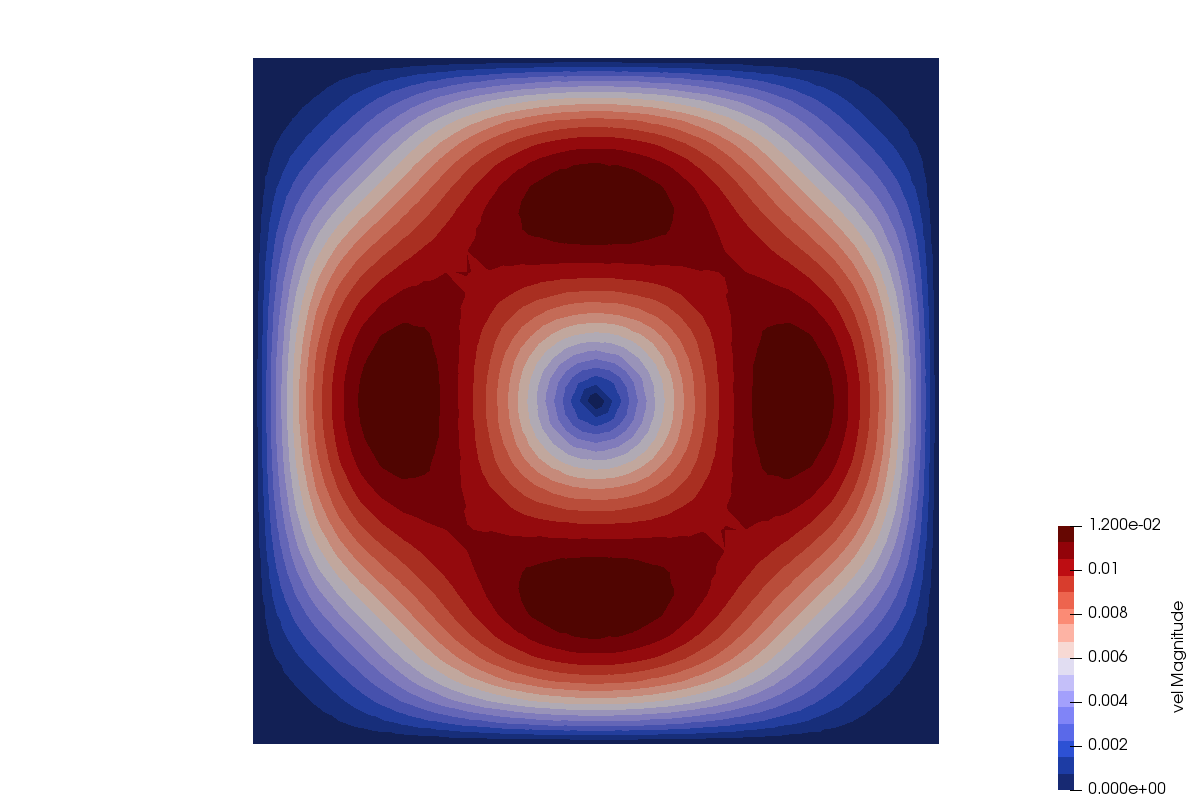
\includegraphics[width=4cm]{python_codes/fieldstone_78/results/mms_dh/16x16/vel0004}
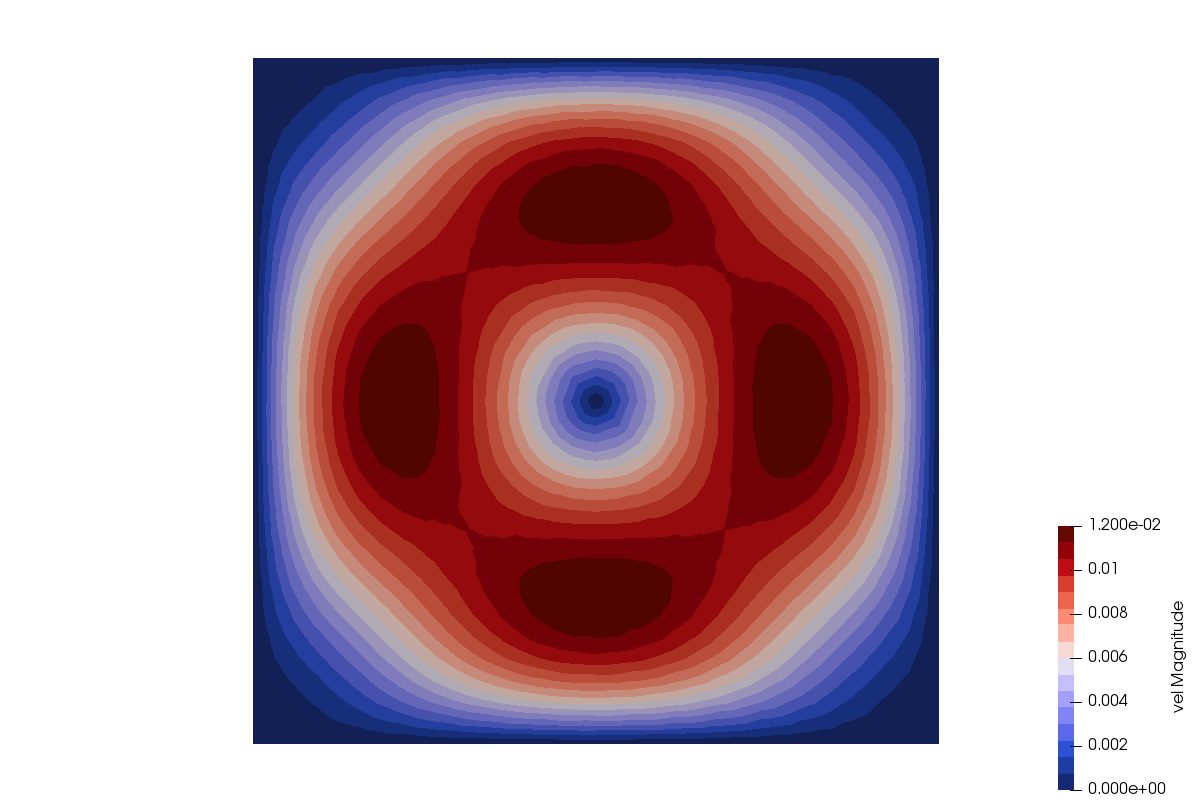
\includegraphics[width=4cm]{python_codes/fieldstone_78/results/mms_dh/16x16/vel0005}
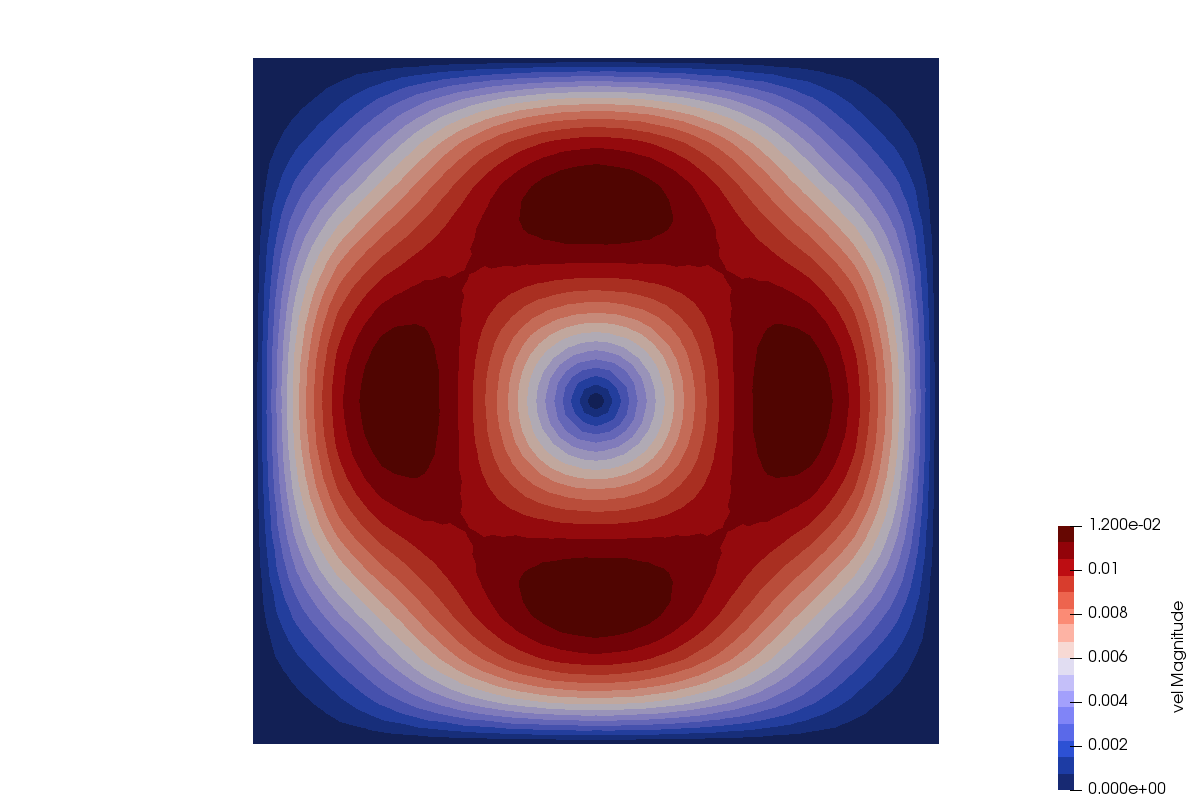
\includegraphics[width=4cm]{python_codes/fieldstone_78/results/mms_dh/16x16/vel0006}
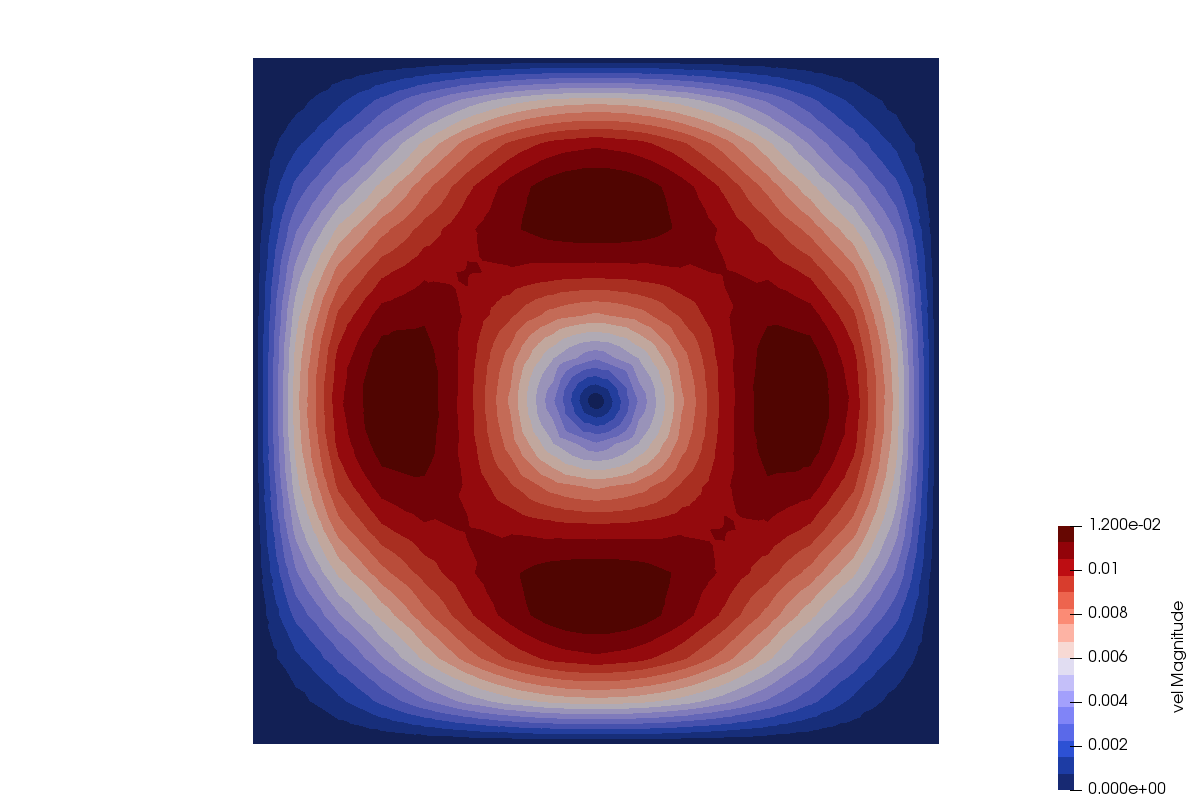
\includegraphics[width=4cm]{python_codes/fieldstone_78/results/mms_dh/16x16/vel0007}\\
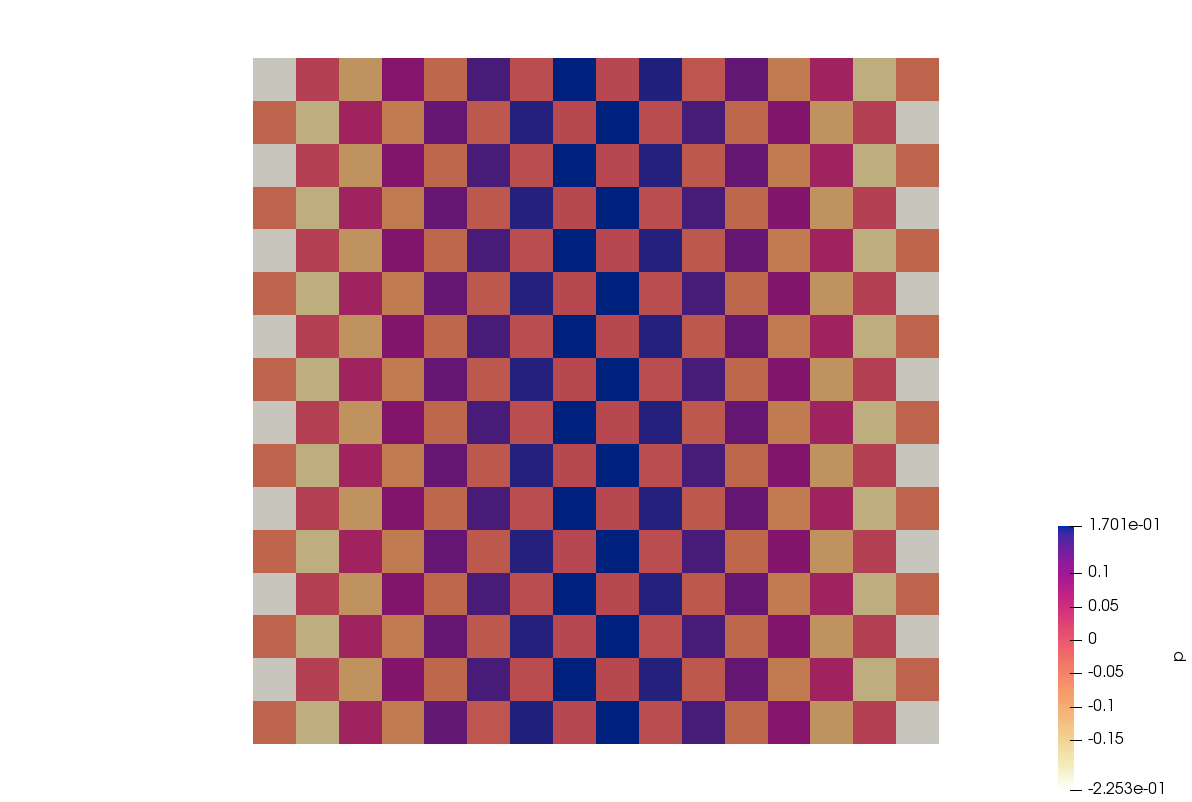
\includegraphics[width=4cm]{python_codes/fieldstone_78/results/mms_dh/16x16/p0}
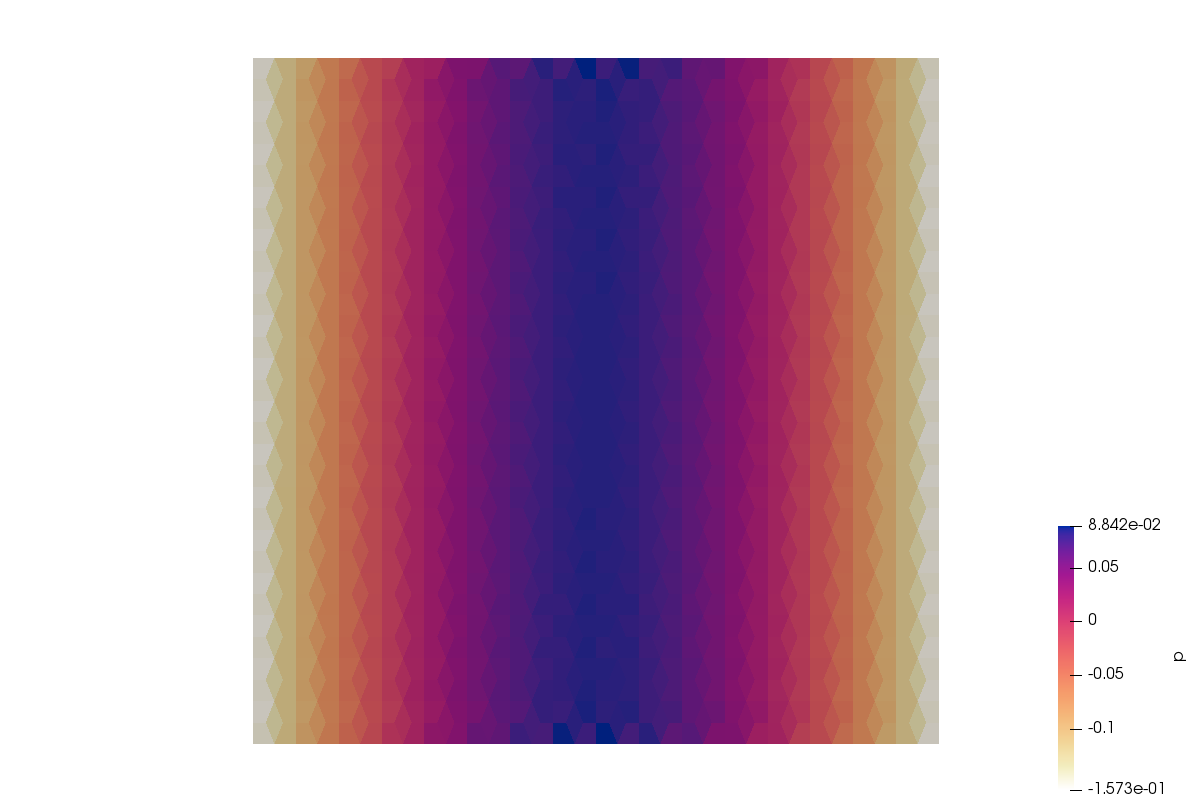
\includegraphics[width=4cm]{python_codes/fieldstone_78/results/mms_dh/16x16/p1}
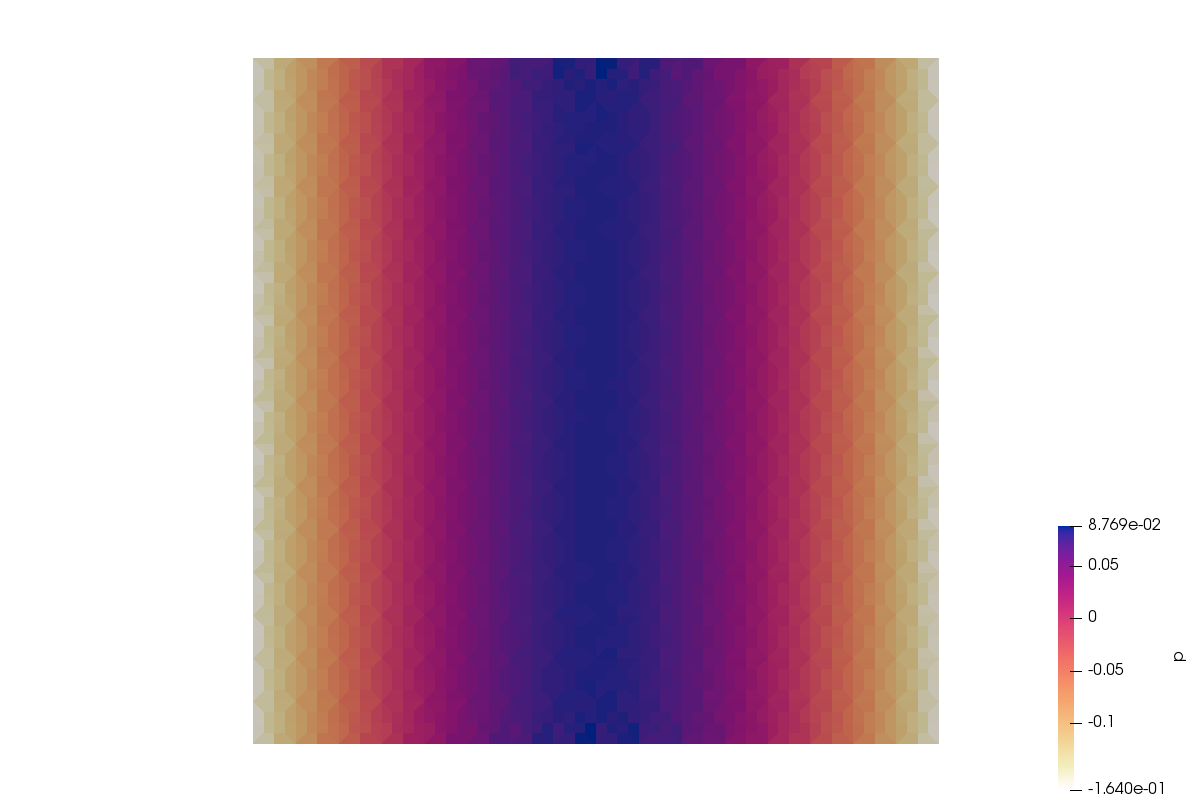
\includegraphics[width=4cm]{python_codes/fieldstone_78/results/mms_dh/16x16/p2}
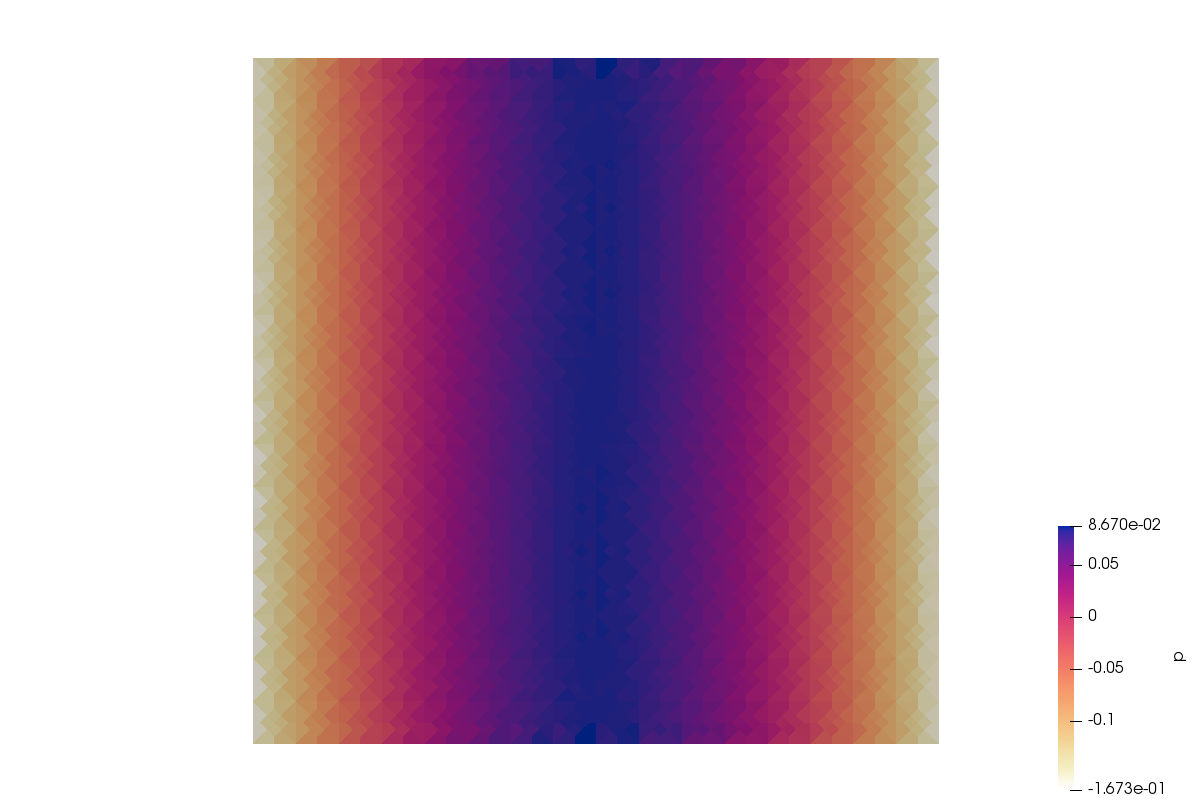
\includegraphics[width=4cm]{python_codes/fieldstone_78/results/mms_dh/16x16/p3}\\
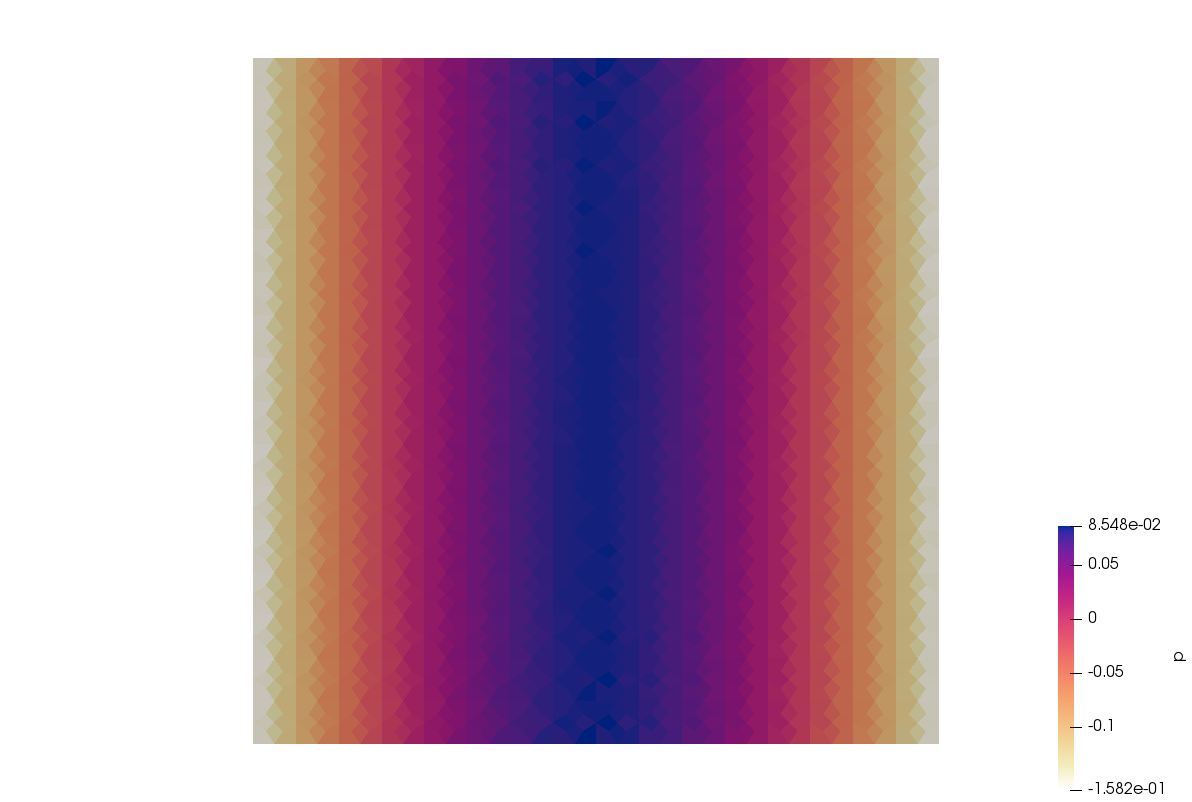
\includegraphics[width=4cm]{python_codes/fieldstone_78/results/mms_dh/16x16/p4}
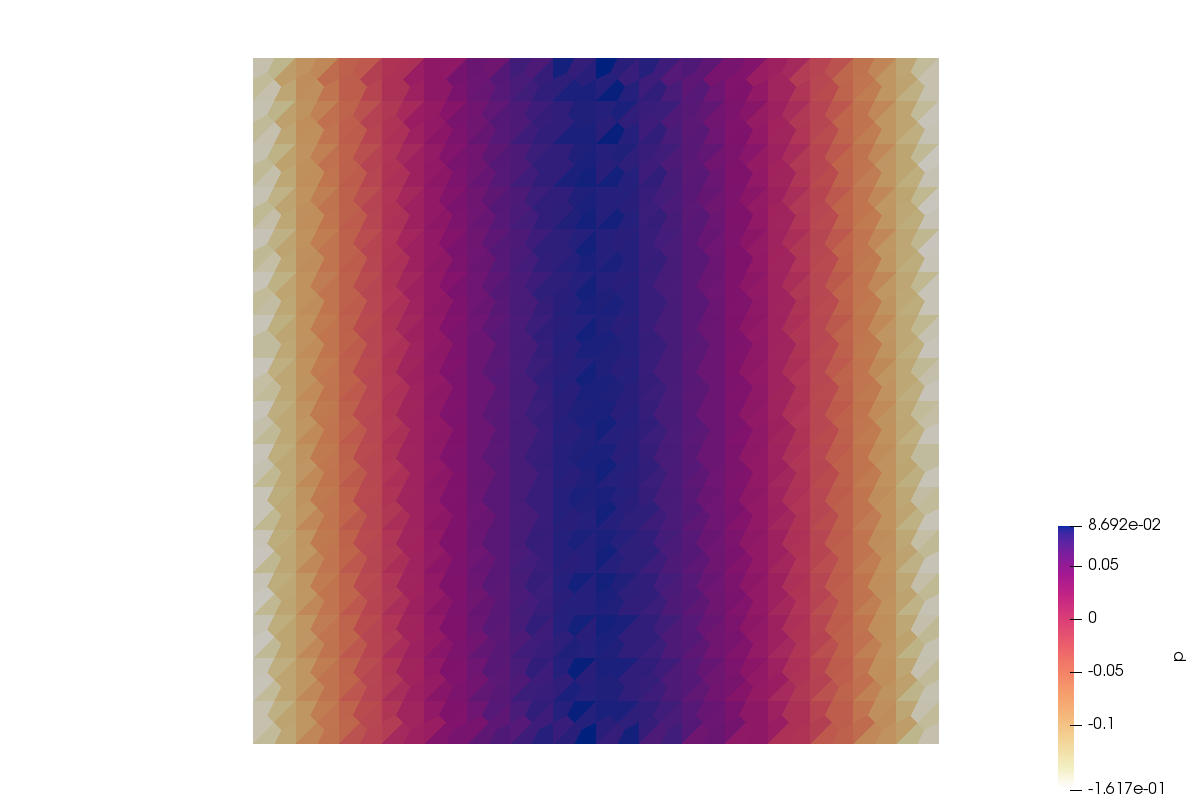
\includegraphics[width=4cm]{python_codes/fieldstone_78/results/mms_dh/16x16/p5}
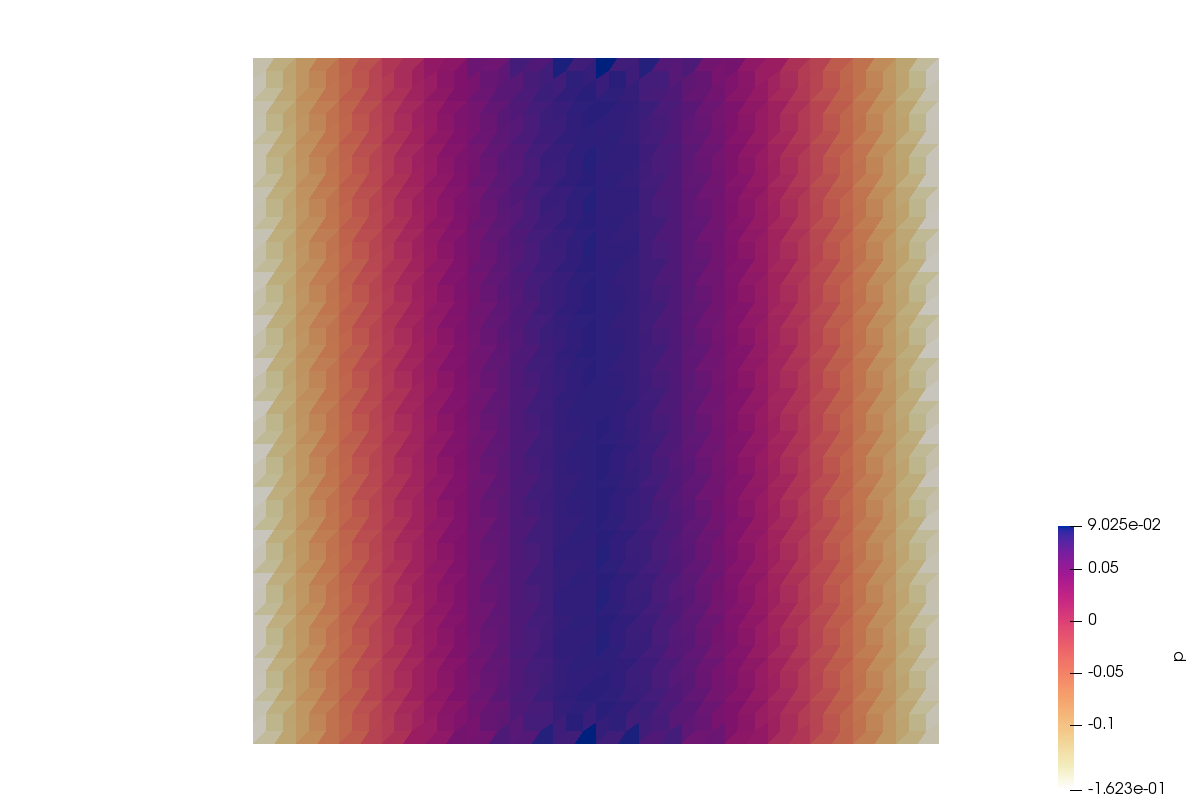
\includegraphics[width=4cm]{python_codes/fieldstone_78/results/mms_dh/16x16/p6}
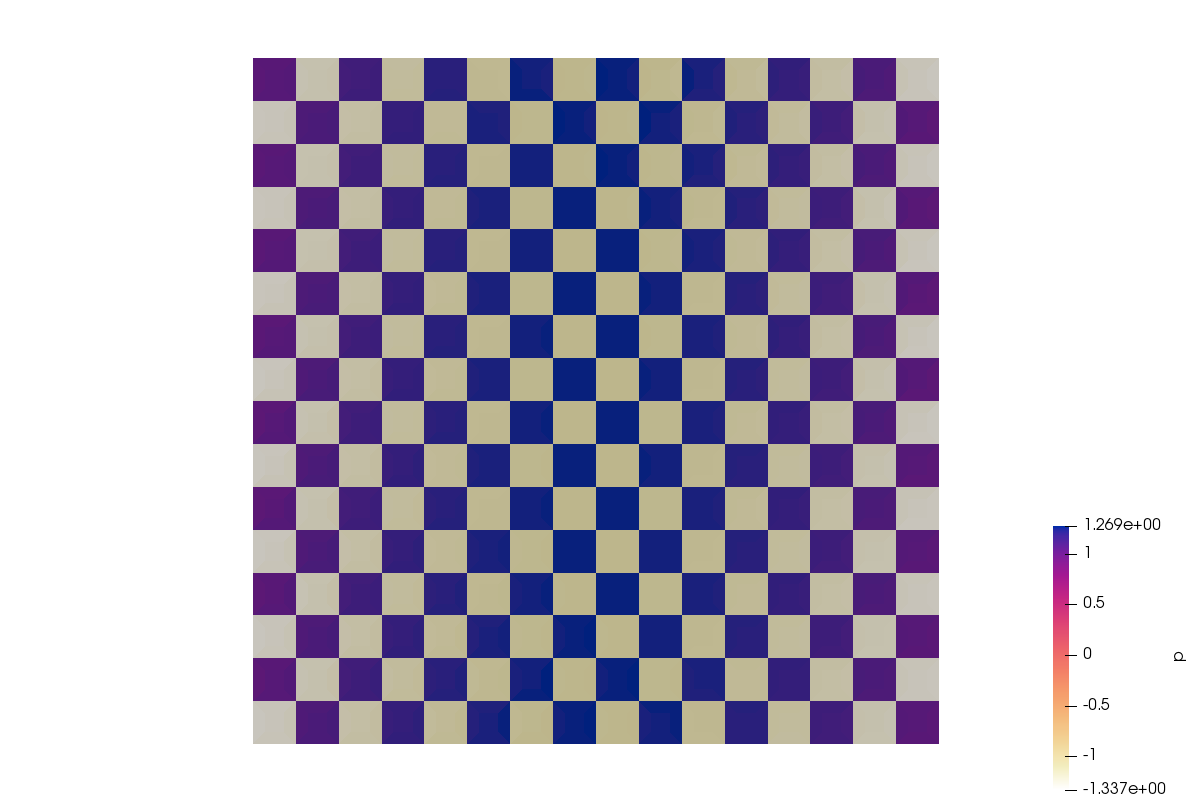
\includegraphics[width=4cm]{python_codes/fieldstone_78/results/mms_dh/16x16/p7}\\
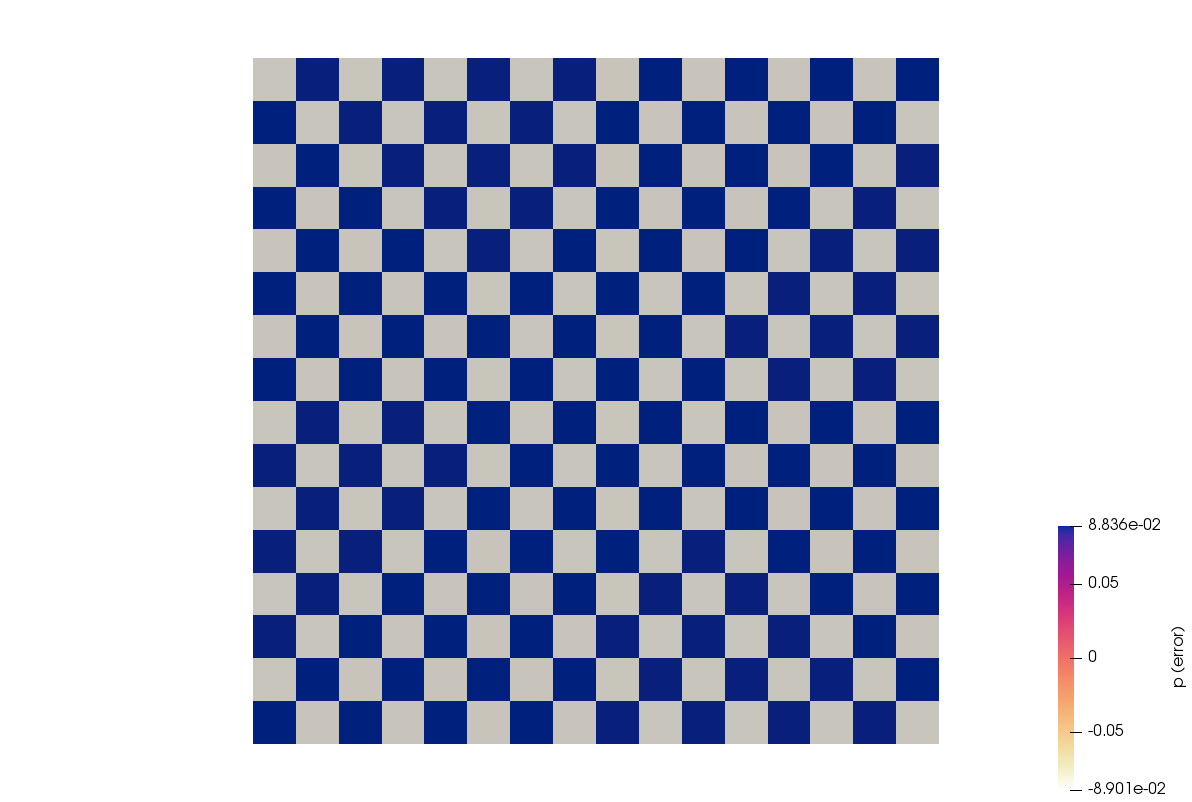
\includegraphics[width=4cm]{python_codes/fieldstone_78/results/mms_dh/16x16/perror0}
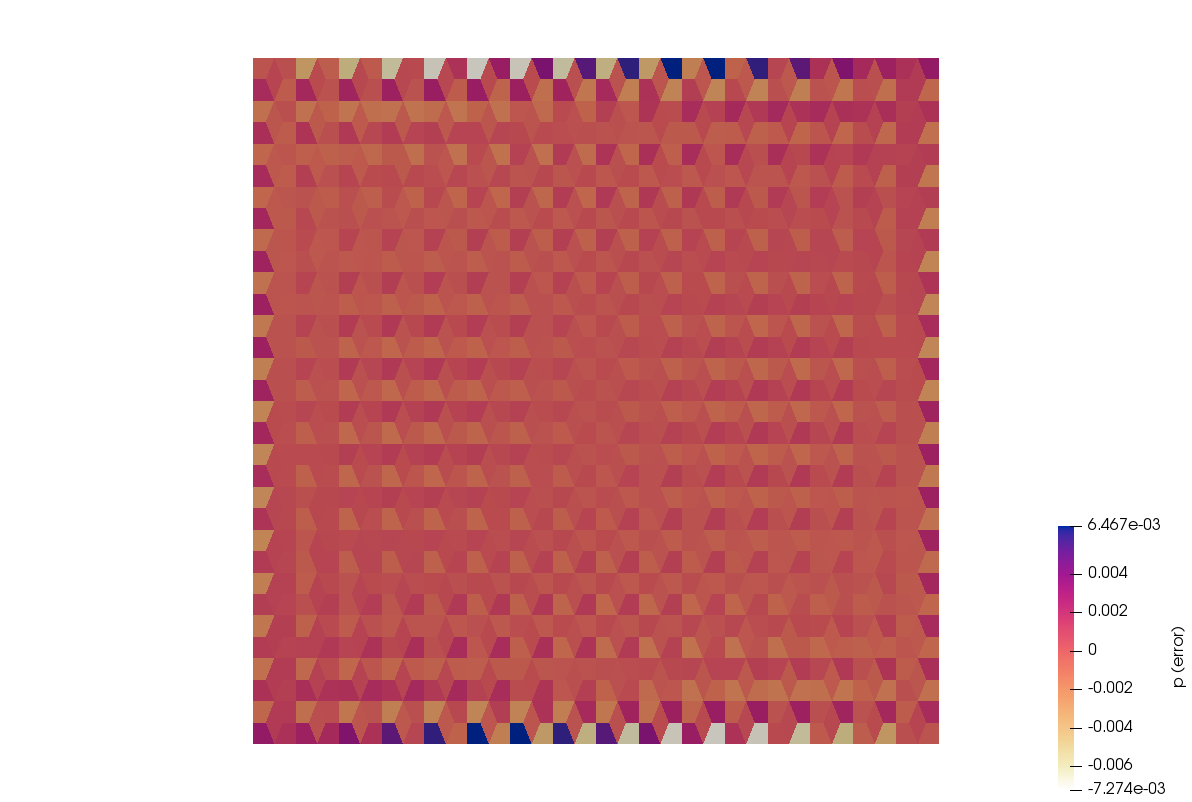
\includegraphics[width=4cm]{python_codes/fieldstone_78/results/mms_dh/16x16/perror1}
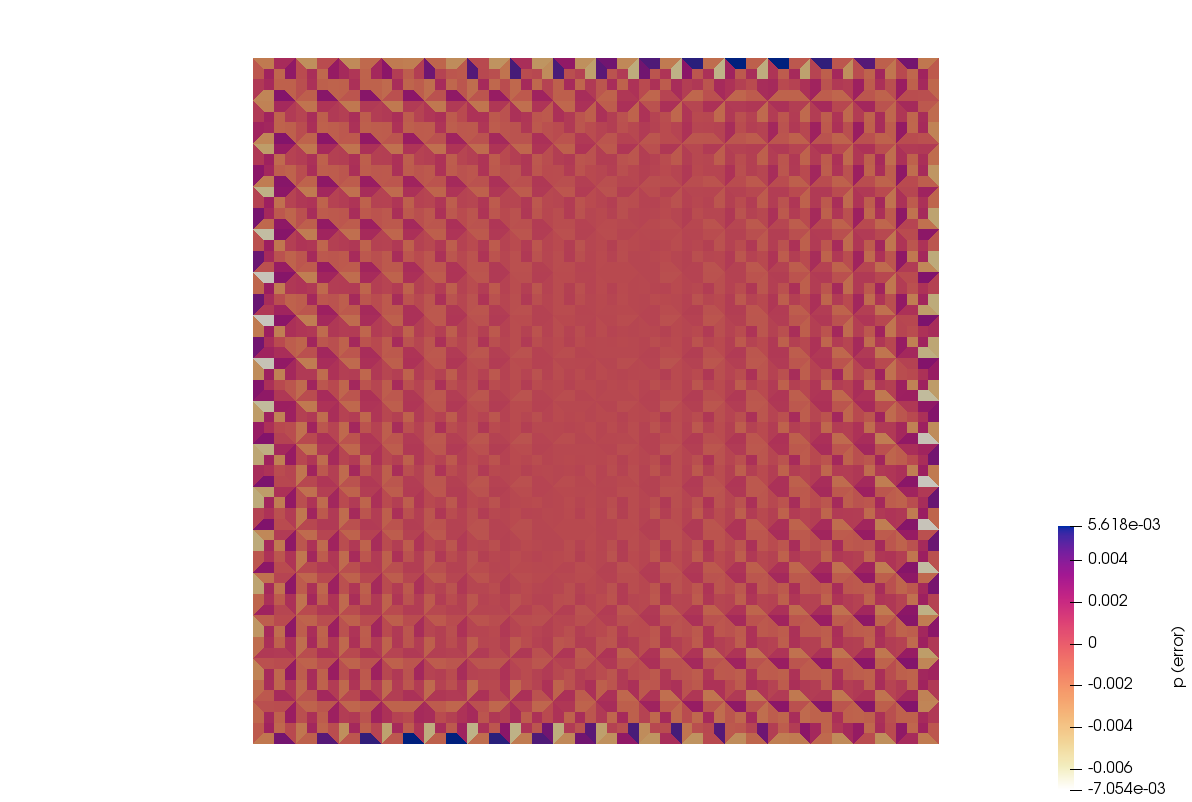
\includegraphics[width=4cm]{python_codes/fieldstone_78/results/mms_dh/16x16/perror2}
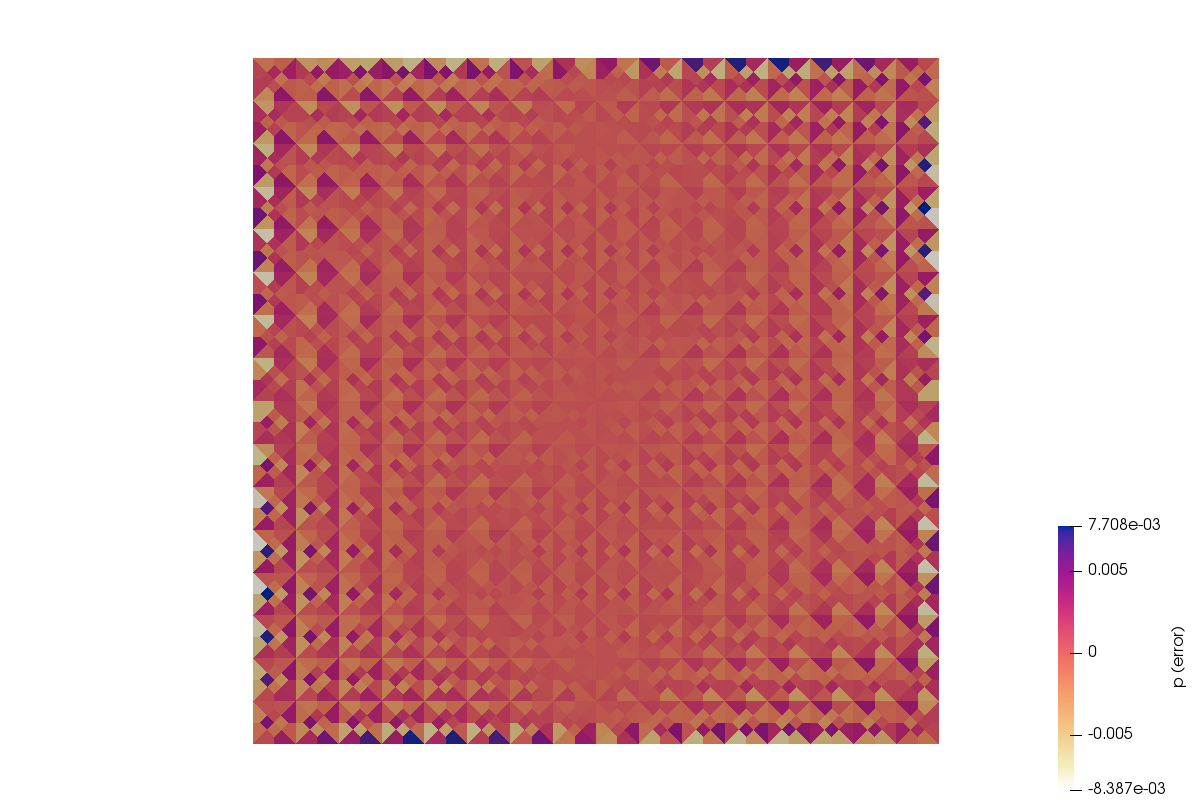
\includegraphics[width=4cm]{python_codes/fieldstone_78/results/mms_dh/16x16/perror3}\\
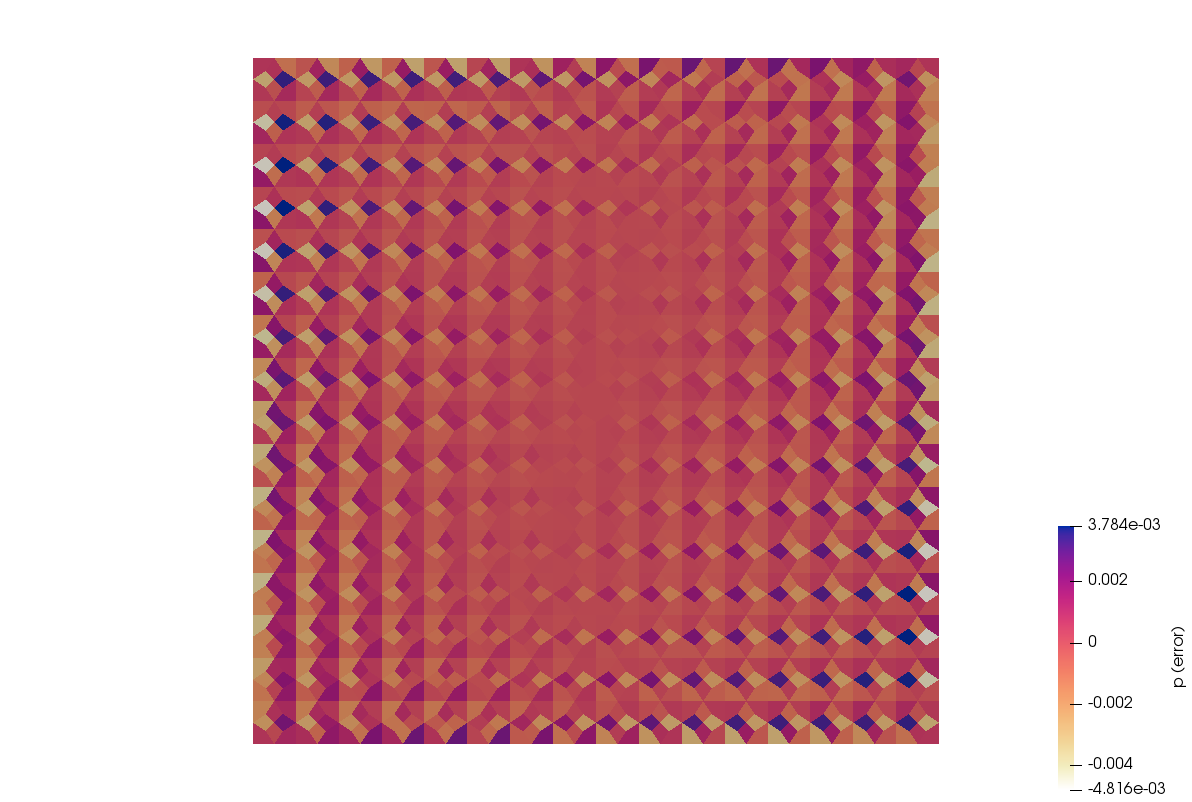
\includegraphics[width=4cm]{python_codes/fieldstone_78/results/mms_dh/16x16/perror4}
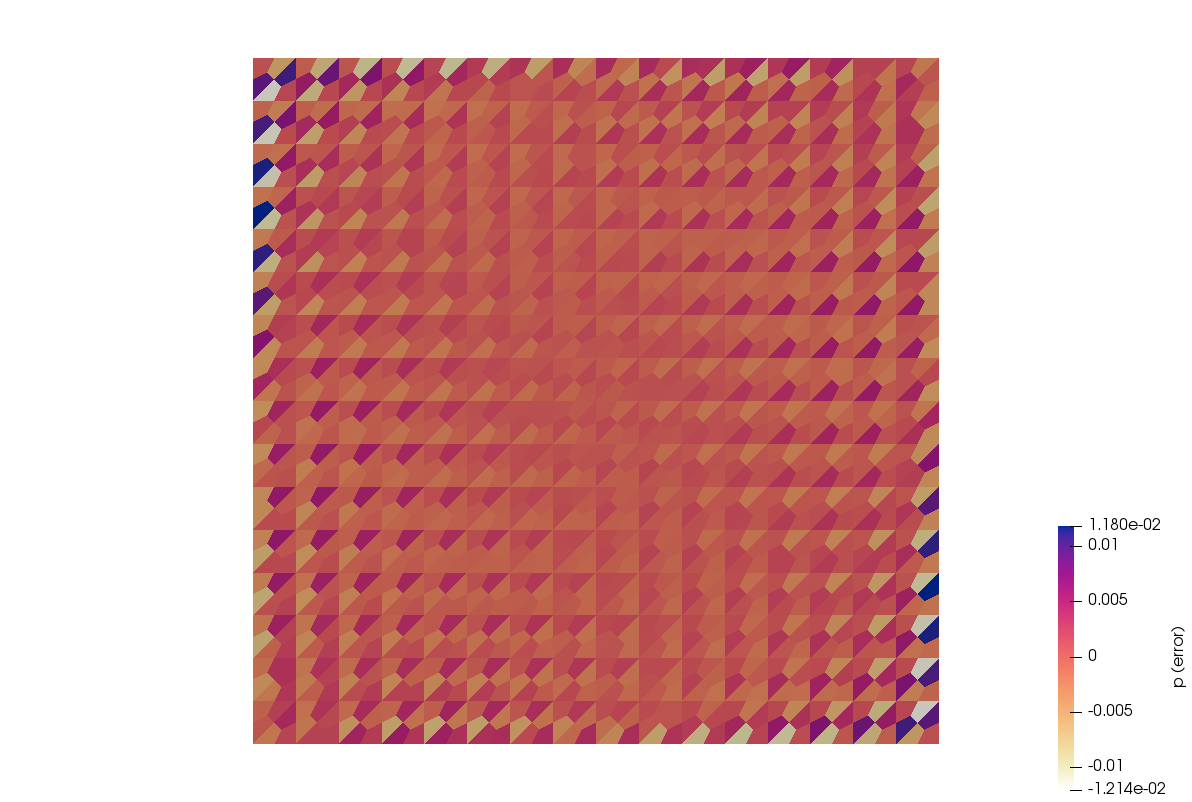
\includegraphics[width=4cm]{python_codes/fieldstone_78/results/mms_dh/16x16/perror5}
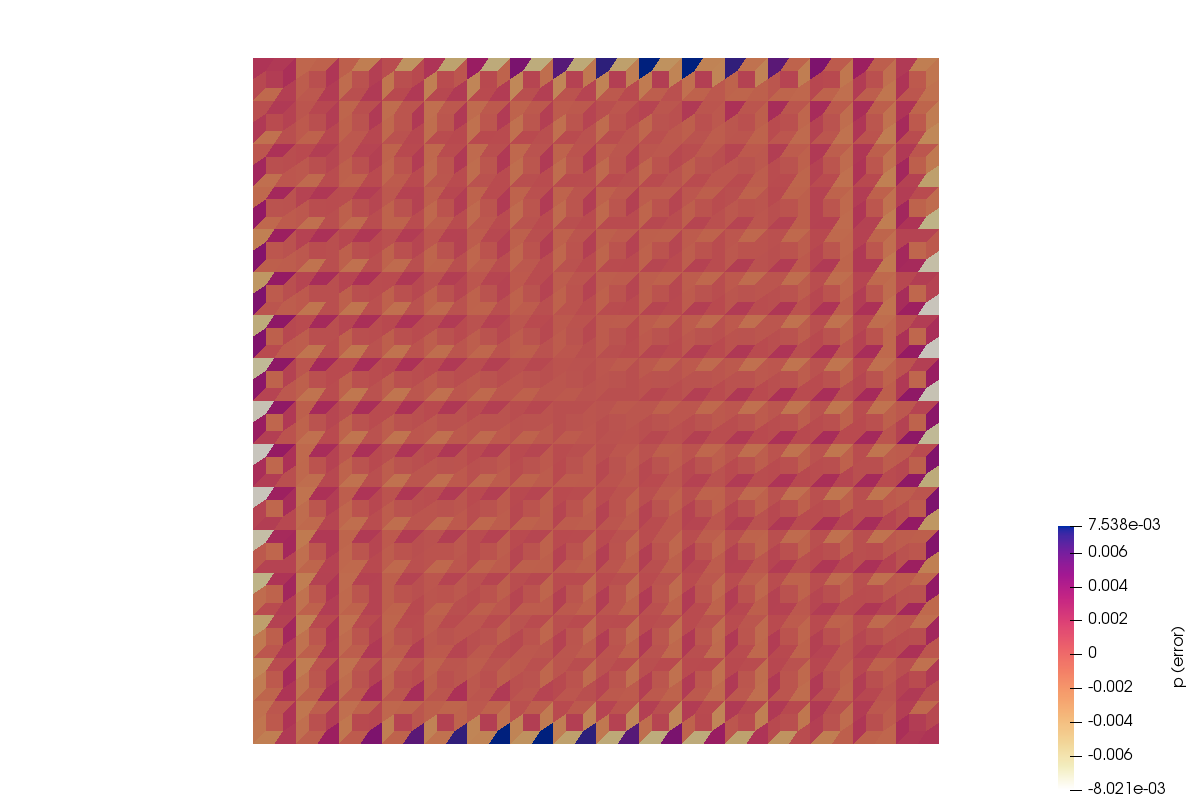
\includegraphics[width=4cm]{python_codes/fieldstone_78/results/mms_dh/16x16/perror6}
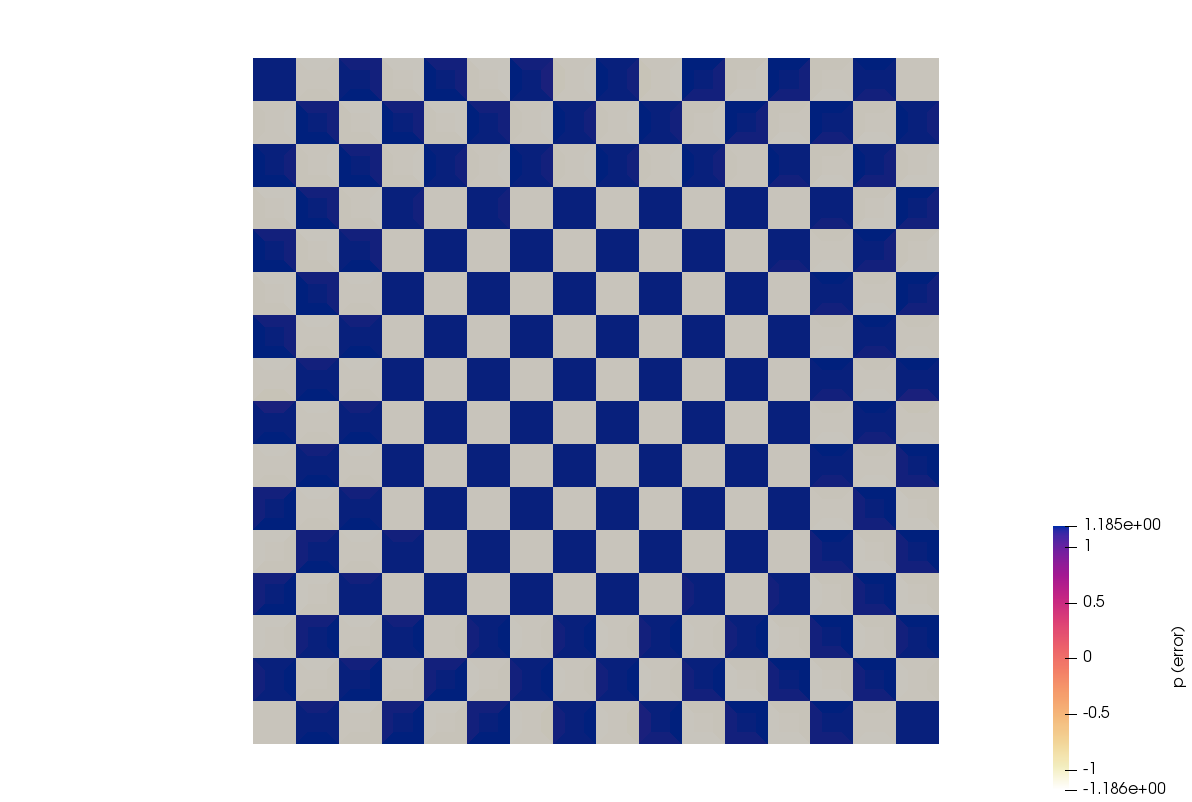
\includegraphics[width=4cm]{python_codes/fieldstone_78/results/mms_dh/16x16/perror7}\\
{\captionfont Meshes  made of 16x16 (macro-)elementscount.} 
\end{center}



Discussion: what is the real advantage of such a macro-element? it is LBB stable, so 
iterative solver will work optimally, and the pressure has no checkerboard. 
Also the number of non-zeros per line of the matrix is small.  
On the other hand it is anisotropic since the 'diamonds are vertical'. 
Also if one would consider a macro-element as an element, it counts 10 velocity nodes and 5 pressures, 
which makes it much more expensive than a $Q_2\times Q_1$ element of the same size...






\newpage
%..................................
\paragraph{Results - Aquarium}


\begin{center}
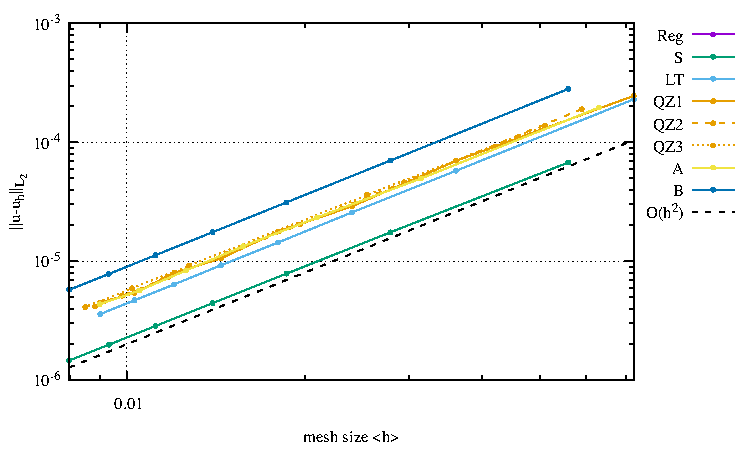
\includegraphics[width=5cm]{python_codes/fieldstone_78/results/aquarium/errors_V}
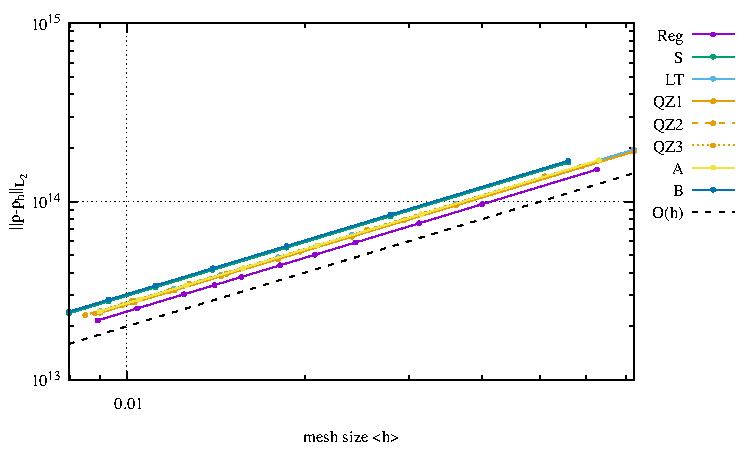
\includegraphics[width=5cm]{python_codes/fieldstone_78/results/aquarium/errors_P}
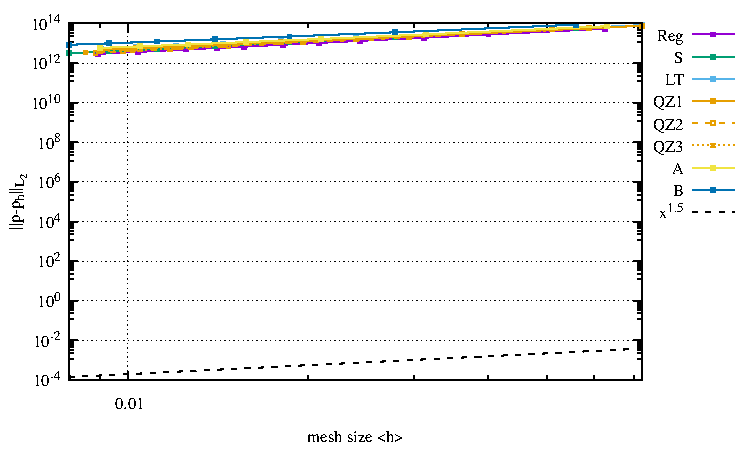
\includegraphics[width=5cm]{python_codes/fieldstone_78/results/aquarium/errors_Q}\\
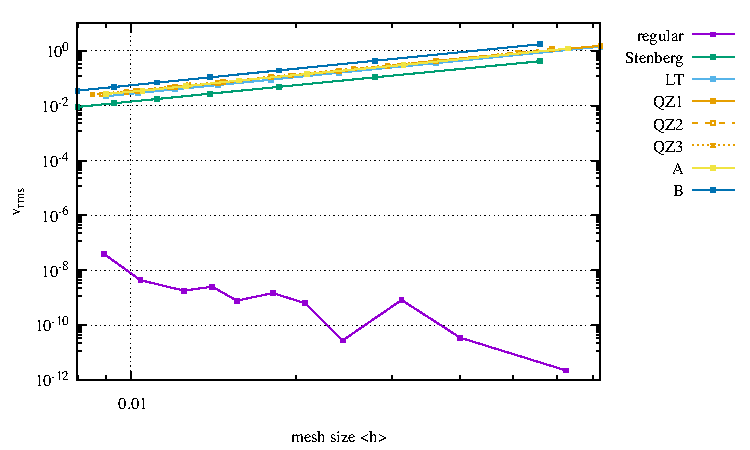
\includegraphics[width=8cm]{python_codes/fieldstone_78/results/aquarium/vrms.pdf}
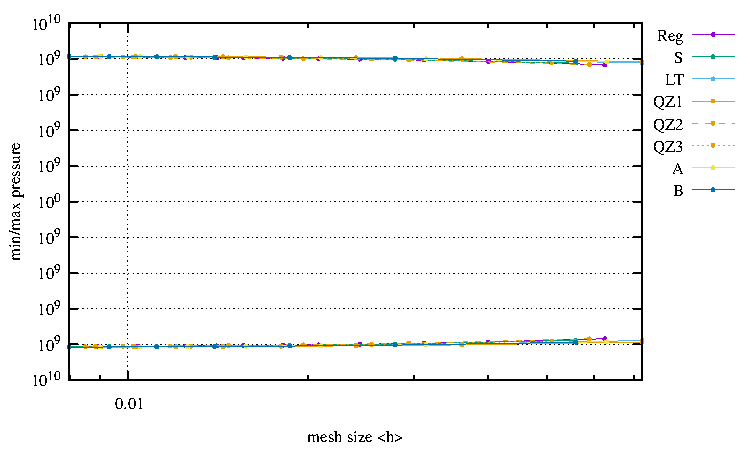
\includegraphics[width=8cm]{python_codes/fieldstone_78/results/aquarium/pstats.pdf}
\end{center}

We see that the Stenberg macro-element is the best, with the lowest velocity and pressure errors.


\newpage
%.....................................................
\paragraph{Results - sinking block - reduced density}

The block has size $0.25\times 0.25$, centered in the domain. No-slip boundary conditions are imposed on all 
sides. The buoyancy force $\rho g_y$ is -1 in the block and zero elsewhere. Viscosity is constant and 
equal to 1 everywhere. 

\begin{center}
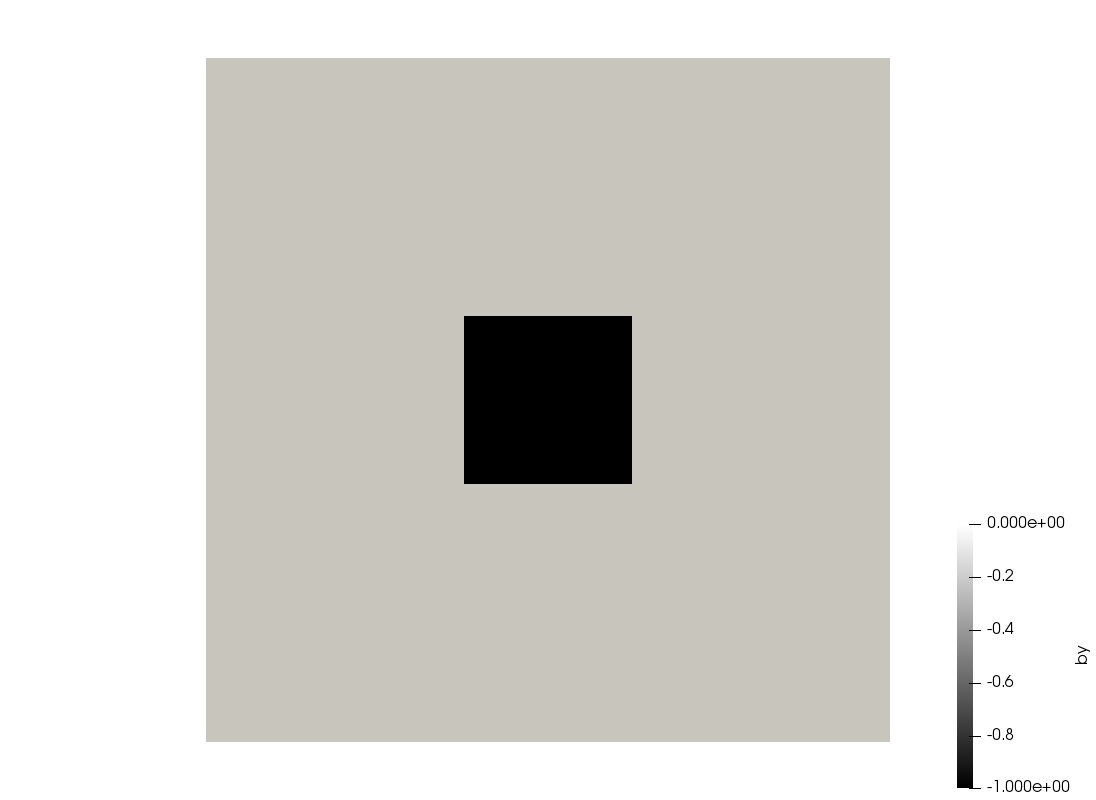
\includegraphics[width=4cm]{python_codes/fieldstone_78/results/sinking_block/reduced/by0}
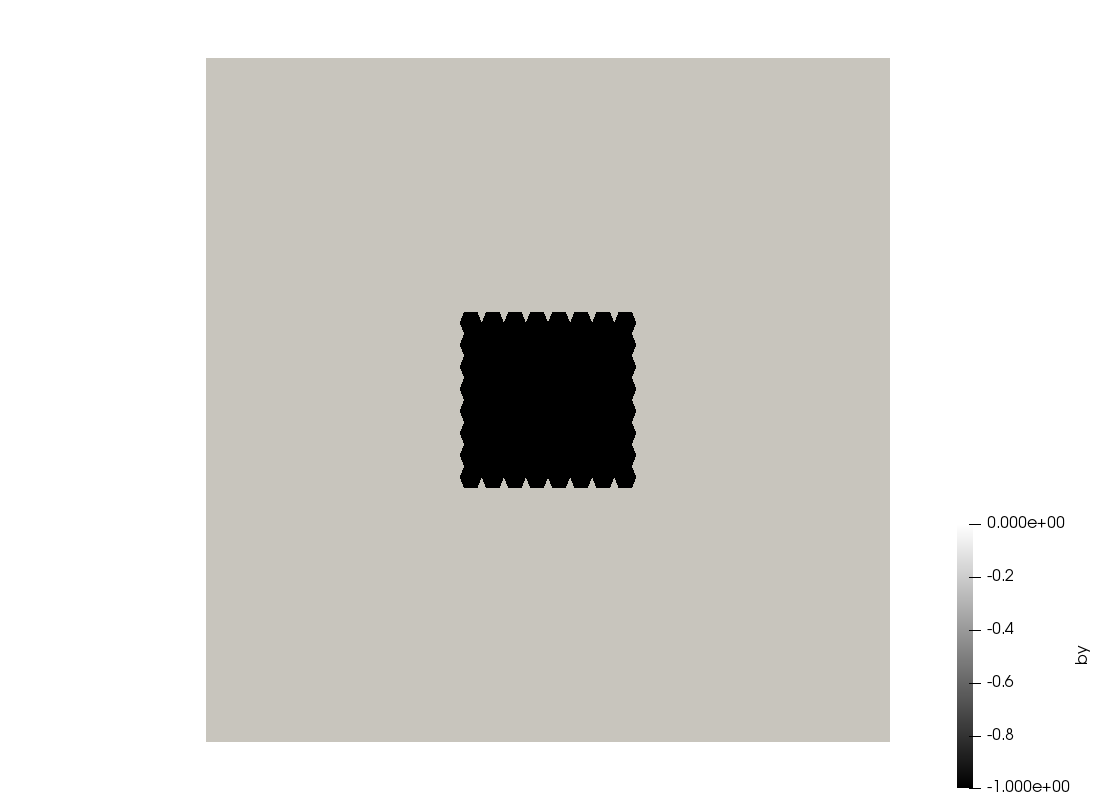
\includegraphics[width=4cm]{python_codes/fieldstone_78/results/sinking_block/reduced/by1}
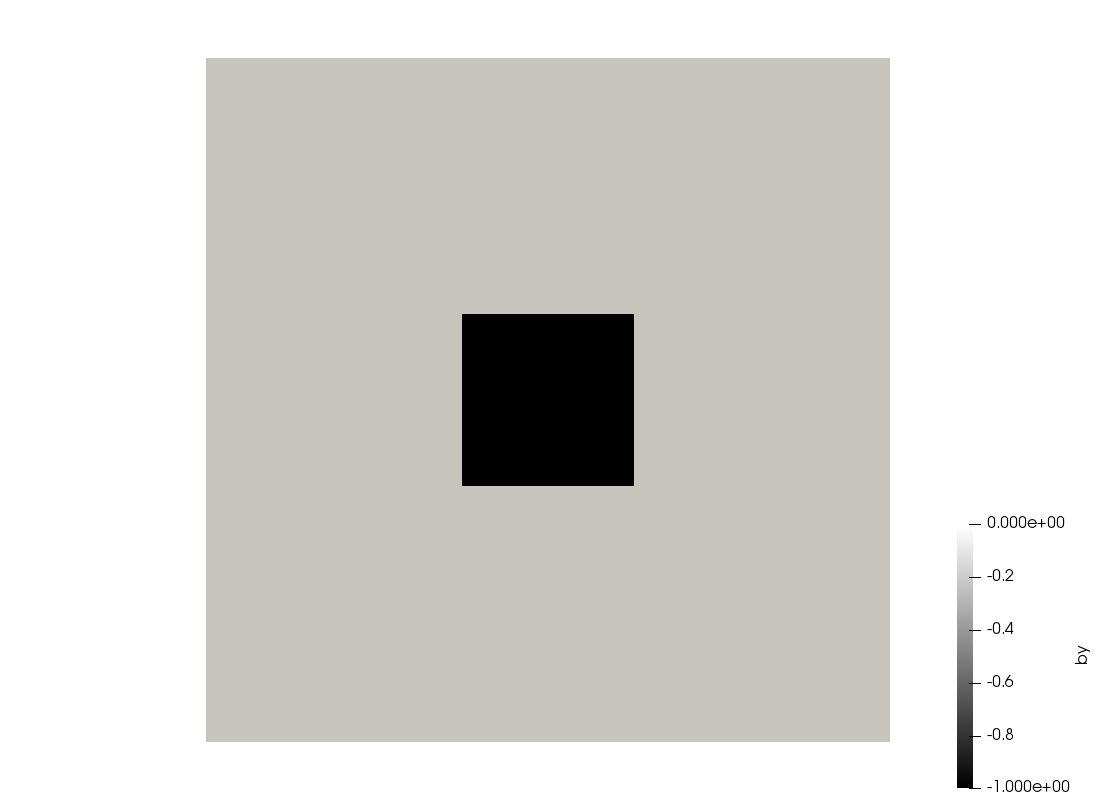
\includegraphics[width=4cm]{python_codes/fieldstone_78/results/sinking_block/reduced/by2}
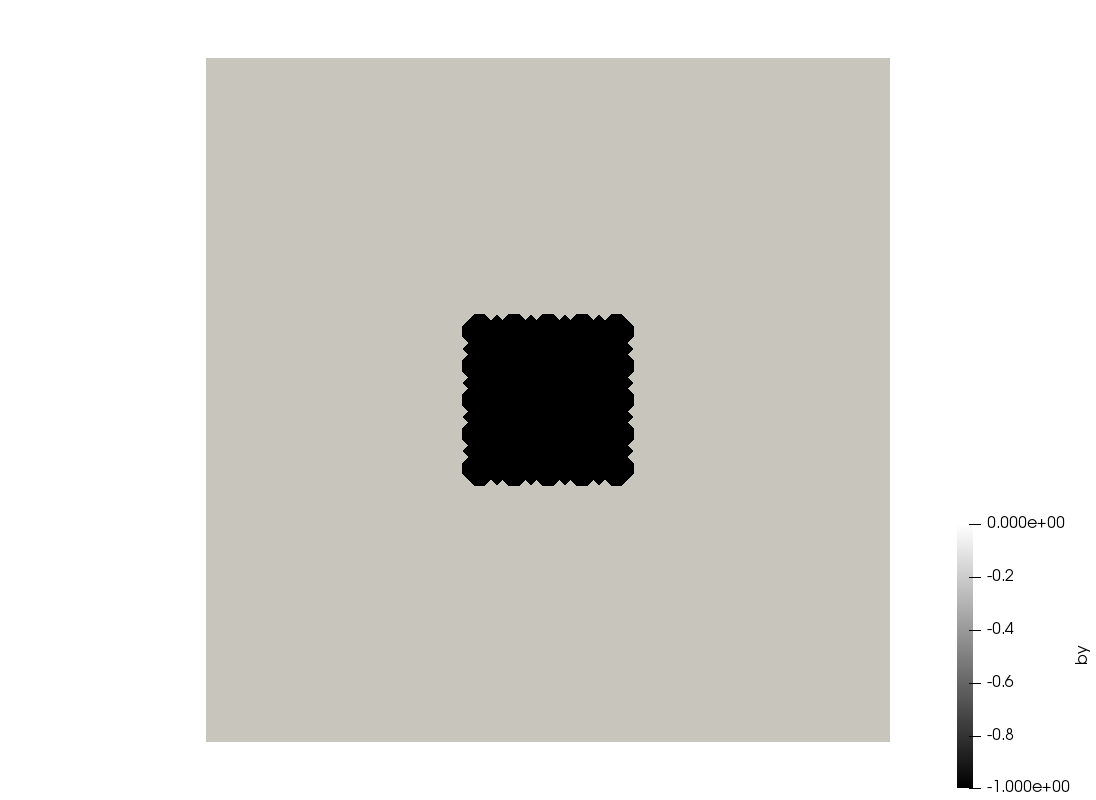
\includegraphics[width=4cm]{python_codes/fieldstone_78/results/sinking_block/reduced/by3}\\
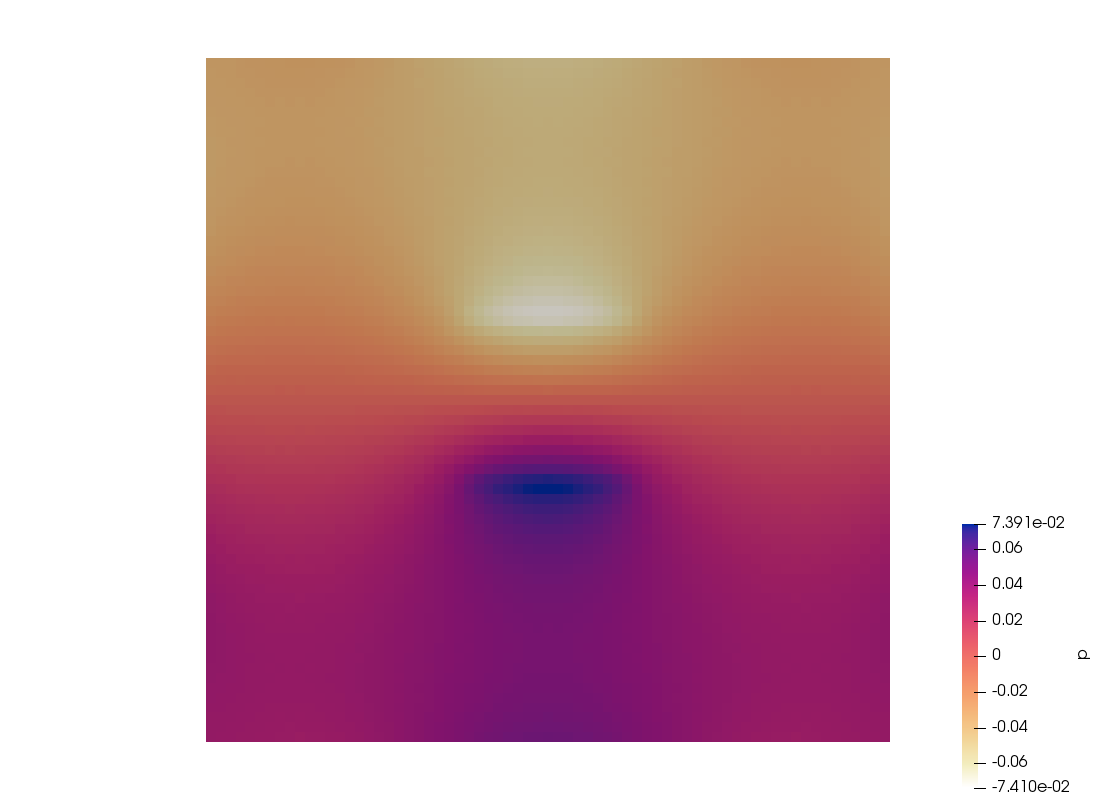
\includegraphics[width=4cm]{python_codes/fieldstone_78/results/sinking_block/reduced/p0}
\includegraphics[width=4cm]{python_codes/fieldstone_78/results/sinking_block/reduced/p1}
\includegraphics[width=4cm]{python_codes/fieldstone_78/results/sinking_block/reduced/p2}
\includegraphics[width=4cm]{python_codes/fieldstone_78/results/sinking_block/reduced/p3}\\
{\captionfont Velocity field (top row) and pressure field (bottom row) 
for regular, Stenberg, Le Tallec, Qin \& Zhang.} 
\end{center}


%.....................................................
\paragraph{Results - sinking block - full density}

We then proceed with $\rho g_y=-1$ in the surrounding fluid and $\rho g_y=-(1+\delta)$ in the block.

%\begin{center}
%\includegraphics[width=3.8cm]{python_codes/fieldstone_78/results/sinking_block/full/vel0}
%\includegraphics[width=3.8cm]{python_codes/fieldstone_78/results/sinking_block/full/vel1}
%\includegraphics[width=3.8cm]{python_codes/fieldstone_78/results/sinking_block/full/vel2}
%\includegraphics[width=3.8cm]{python_codes/fieldstone_78/results/sinking_block/full/vel3}\\
%\includegraphics[width=3.8cm]{python_codes/fieldstone_78/results/sinking_block/full/p0}
%\includegraphics[width=3.8cm]{python_codes/fieldstone_78/results/sinking_block/full/p1}
%\includegraphics[width=3.8cm]{python_codes/fieldstone_78/results/sinking_block/full/p2}
%\includegraphics[width=3.8cm]{python_codes/fieldstone_78/results/sinking_block/full/p3}\\
%{\captionfont buoyancy term $b_y$; pressure field for regular, Stenberg, Le Tallec, Qin \& Zhang.} 
%\end{center}


\newpage
%..................................
\paragraph{Results - Stokes sphere}

This is the same experiment as above, except for the geometry of the object 
which is now a sphere of radius 0.125 so that the interface between both fluids 
is never aligned with the mesh/element edges. The sphere has density is 1 while the surrounding is 0.
Its viscosity is $10^4$ while the surrounding is 1.


\begin{center}
\includegraphics[width=5cm]{python_codes/fieldstone_78/results/sphere/ustats}
\includegraphics[width=5cm]{python_codes/fieldstone_78/results/sphere/vstats}
\includegraphics[width=5cm]{python_codes/fieldstone_78/results/sphere/vrms.pdf}\\
\includegraphics[width=7cm]{python_codes/fieldstone_78/results/sphere/pstats.pdf}
\includegraphics[width=7cm]{python_codes/fieldstone_78/results/sphere/qstats}
\end{center}



All (macro-)elements converge to the same vrms and show very similar velocity and pressure statistics.
Stenberg is undeniably the best in terms of pressure under/over shoot. 



\newpage
%..................................
\paragraph{Results - Regularised lid driven cavity}

Domain is 1x1. Viscosity is 1 and density is zero. 
No-slip prescribed at sides and bottom and $\vec{\upnu}=(16x^2(1-x^2),0)$ prescribed on the top.


\begin{center}
\includegraphics[width=6cm]{python_codes/fieldstone_78/results/ldc/32x32/vel}
\includegraphics[width=6cm]{python_codes/fieldstone_78/results/ldc/32x32/vel2}\\
\includegraphics[width=6cm]{python_codes/fieldstone_78/results/ldc/32x32/u}
\includegraphics[width=6cm]{python_codes/fieldstone_78/results/ldc/32x32/v}\\
\includegraphics[width=6cm]{python_codes/fieldstone_78/results/ldc/32x32/p0}
\includegraphics[width=6cm]{python_codes/fieldstone_78/results/ldc/32x32/p1}\\
\includegraphics[width=6cm]{python_codes/fieldstone_78/results/ldc/32x32/p2}
\includegraphics[width=6cm]{python_codes/fieldstone_78/results/ldc/32x32/p3}\\
\includegraphics[width=6cm]{python_codes/fieldstone_78/results/ldc/32x32/p4}
\includegraphics[width=6cm]{python_codes/fieldstone_78/results/ldc/32x32/p5}\\
\includegraphics[width=6cm]{python_codes/fieldstone_78/results/ldc/32x32/p6}
\includegraphics[width=6cm]{python_codes/fieldstone_78/results/ldc/32x32/p7}\\
{\captionfont 32x32 mesh. Note the insane amplitude of the checkerboard modes!}
\end{center}

\begin{center}
\includegraphics[width=7cm]{python_codes/fieldstone_78/results/ldc/ustats}
\includegraphics[width=7cm]{python_codes/fieldstone_78/results/ldc/vstats}\\
\includegraphics[width=7cm]{python_codes/fieldstone_78/results/ldc/pstats.pdf}
\includegraphics[width=7cm]{python_codes/fieldstone_78/results/ldc/vrms.pdf}
\end{center}

\begin{center}
\includegraphics[width=7cm]{python_codes/fieldstone_78/results/ldc/32x32/prop}
\includegraphics[width=7cm]{python_codes/fieldstone_78/results/ldc/32x32/vel_profile}\\
{\captionfont Left: Pressure at the surface; Right: velocity on vertical line in the middle}
\end{center}

\newpage
%......................................
\paragraph{Results - analytical cavity}

\begin{center}
\includegraphics[width=5cm]{python_codes/fieldstone_78/results/mms_cavity/ustats}
\includegraphics[width=5cm]{python_codes/fieldstone_78/results/mms_cavity/vstats}
\includegraphics[width=5cm]{python_codes/fieldstone_78/results/mms_cavity/vrms.pdf}\\
\includegraphics[width=7cm]{python_codes/fieldstone_78/results/mms_cavity/pstats.pdf}
\includegraphics[width=7cm]{python_codes/fieldstone_78/results/mms_cavity/qstats}
\end{center}

\begin{center}
\includegraphics[width=7cm]{python_codes/fieldstone_78/results/mms_cavity/32x32/prop}
\includegraphics[width=7cm]{python_codes/fieldstone_78/results/mms_cavity/32x32/vel_profile}
\end{center}


\newpage
%......................................
\paragraph{Results - SolKz}

\begin{center}
\includegraphics[width=5cm]{python_codes/fieldstone_78/results/mms_solkz/errors_V}
\includegraphics[width=5cm]{python_codes/fieldstone_78/results/mms_solkz/errors_P}
\includegraphics[width=5cm]{python_codes/fieldstone_78/results/mms_solkz/errors_Q}\\
\includegraphics[width=5cm]{python_codes/fieldstone_78/results/mms_solkz/ustats}
\includegraphics[width=5cm]{python_codes/fieldstone_78/results/mms_solkz/vstats}
\includegraphics[width=5cm]{python_codes/fieldstone_78/results/mms_solkz/vrms.pdf}\\
\includegraphics[width=7cm]{python_codes/fieldstone_78/results/mms_solkz/pstats.pdf}
\includegraphics[width=7cm]{python_codes/fieldstone_78/results/mms_solkz/qstats}
\end{center}

\begin{center}
\includegraphics[width=7cm]{python_codes/fieldstone_78/results/mms_solkz/32x32/prop}
\includegraphics[width=7cm]{python_codes/fieldstone_78/results/mms_solkz/32x32/vel_profile}
\end{center}

\newpage
%......................................
\paragraph{Results - square cylinder}

This experiment is inspired by the very common one found in CFD: a laminar flow 
is forced to go around a cylinder (circular or square cross section) often 
generating turbulence in its wake for high-enough Reynolds number Navier-Stokes flow.

The domain is 4x1. Free slip boundary conditions are imposed top and bottom. 
A horizontal flow $\vec{v}=(0,1)$ is prescribed on the left boundary, and the 
right boundary is left open. All the nodes on a square centered in the middle of the domain 
of size 0.125x0.125 are set to no-slip boundary conditions.
Viscosity is one and gravity is switched off.

\begin{center}
\includegraphics[width=7cm]{python_codes/fieldstone_78/results/cylinder/vel}
\includegraphics[width=7cm]{python_codes/fieldstone_78/results/cylinder/vel2}\\
\includegraphics[width=7cm]{python_codes/fieldstone_78/results/cylinder/u}
\includegraphics[width=7cm]{python_codes/fieldstone_78/results/cylinder/v}\\
\includegraphics[width=7cm]{python_codes/fieldstone_78/results/cylinder/p0}
\includegraphics[width=7cm]{python_codes/fieldstone_78/results/cylinder/p1}\\
\includegraphics[width=7cm]{python_codes/fieldstone_78/results/cylinder/p2}
\includegraphics[width=7cm]{python_codes/fieldstone_78/results/cylinder/p3}\\
\includegraphics[width=7cm]{python_codes/fieldstone_78/results/cylinder/p4}
\includegraphics[width=7cm]{python_codes/fieldstone_78/results/cylinder/p5}\\
\includegraphics[width=7cm]{python_codes/fieldstone_78/results/cylinder/p6}
\includegraphics[width=7cm]{python_codes/fieldstone_78/results/cylinder/p7}
\end{center}

run with script\_cylinder

\newpage
%.........................................................
\paragraph{Results - flow over a cavity (experiment=11)}

The domain is 4x1. No slip boundary conditions are imposed on all walls.
The cavity is formed by prescribing $\vec{\upnu}=\vec{0}$ on the right
nodes inside the domain. $\vec{\upnu}=-(y-L_y)(y-L_y/2)$ is prescribed 
on the left inflow boundary while $\upnu_y=0$ is prescribed on the outflow boundary.
Viscosity is one and gravity is switched off.
 
\begin{center}
\includegraphics[width=7cm]{python_codes/fieldstone_78/results/flow_over_cavity/vel}
\includegraphics[width=7cm]{python_codes/fieldstone_78/results/flow_over_cavity/vel2}\\
\includegraphics[width=7cm]{python_codes/fieldstone_78/results/flow_over_cavity/u}
\includegraphics[width=7cm]{python_codes/fieldstone_78/results/flow_over_cavity/v}\\
\includegraphics[width=7cm]{python_codes/fieldstone_78/results/flow_over_cavity/p0}
\includegraphics[width=7cm]{python_codes/fieldstone_78/results/flow_over_cavity/p1}\\
\includegraphics[width=7cm]{python_codes/fieldstone_78/results/flow_over_cavity/p2}
\includegraphics[width=7cm]{python_codes/fieldstone_78/results/flow_over_cavity/p3}\\
\includegraphics[width=7cm]{python_codes/fieldstone_78/results/flow_over_cavity/p4}
\includegraphics[width=7cm]{python_codes/fieldstone_78/results/flow_over_cavity/p5}\\
\includegraphics[width=7cm]{python_codes/fieldstone_78/results/flow_over_cavity/p6}
\includegraphics[width=7cm]{python_codes/fieldstone_78/results/flow_over_cavity/p7}
\end{center}

run with script\_cavity




\newpage
%.........................................................
\paragraph{Results - flow over an obstacle (experiment=12)}

Domain is 4x1. Viscosity is 1, $rho g = -1$. Free slip top and bottom.
Obstacle is no slip and is composed of nodes at $x=L_x/2$ and $y\le L_y/2$.
$\vec\upnu=(1,0)$ prescribed on the left, $\upnu_y=0$ on the right.

\begin{center}
\includegraphics[width=7cm]{python_codes/fieldstone_78/results/flow_over_obstacle/vel}
\includegraphics[width=7cm]{python_codes/fieldstone_78/results/flow_over_obstacle/vel2}\\
\includegraphics[width=7cm]{python_codes/fieldstone_78/results/flow_over_obstacle/u}
\includegraphics[width=7cm]{python_codes/fieldstone_78/results/flow_over_obstacle/v}\\
\includegraphics[width=7cm]{python_codes/fieldstone_78/results/flow_over_obstacle/p0}
\includegraphics[width=7cm]{python_codes/fieldstone_78/results/flow_over_obstacle/p1}
\end{center}

run with script\_obstacle
 
\newpage
%.........................................................
\paragraph{Results - SolCx mms (experiment=13)}

Even number of elements:

\begin{center}
\includegraphics[width=7cm]{python_codes/fieldstone_78/results/mms_solcx/even/errors_V}
\includegraphics[width=7cm]{python_codes/fieldstone_78/results/mms_solcx/even/errors_P}\\
\includegraphics[width=7cm]{python_codes/fieldstone_78/results/mms_solcx/even/errors_Q}
\includegraphics[width=7cm]{python_codes/fieldstone_78/results/mms_solcx/even/vrms.pdf}
\end{center}

Odd number of elements:

\begin{center}
\includegraphics[width=7cm]{python_codes/fieldstone_78/results/mms_solcx/odd/errors_V}
\includegraphics[width=7cm]{python_codes/fieldstone_78/results/mms_solcx/odd/errors_P}\\
\includegraphics[width=7cm]{python_codes/fieldstone_78/results/mms_solcx/odd/errors_Q}
\includegraphics[width=7cm]{python_codes/fieldstone_78/results/mms_solcx/odd/vrms.pdf}
\end{center}

\newpage
%.........................................................
\paragraph{Results - Solvi mms (experiment=14)}

\begin{center}
\includegraphics[width=7cm]{python_codes/fieldstone_78/results/mms_solvi/errors_V}
\includegraphics[width=7cm]{python_codes/fieldstone_78/results/mms_solvi/errors_P}\\
\includegraphics[width=7cm]{python_codes/fieldstone_78/results/mms_solvi/errors_Q}
\includegraphics[width=7cm]{python_codes/fieldstone_78/results/mms_solvi/vrms.pdf}
\end{center}














